
\subsection{Details of Cross Section Extraction Procedure} 
\label{Sec:supplementalanalysis}

This section provides more detailed description of the cross section extraction procedure for \tkidelta, starting with the sideband tuning procedure, background subtraction, unfolding, and finally efficiency correction. Figure~\ref{fig:tkidelta_sdbn_evntrate_tuned}  shows the sideband sample with a Michel electron after tuning the backgrounds for events interacting on scintillator and events interacting on lead as a function of \tkidelta.  Note that the background fractions vary significantly between scintillator and lead, underscoring the importance of measuring backgrounds for each target nucleus separately wherever possible.  

\begin{figure}  
	\centering
	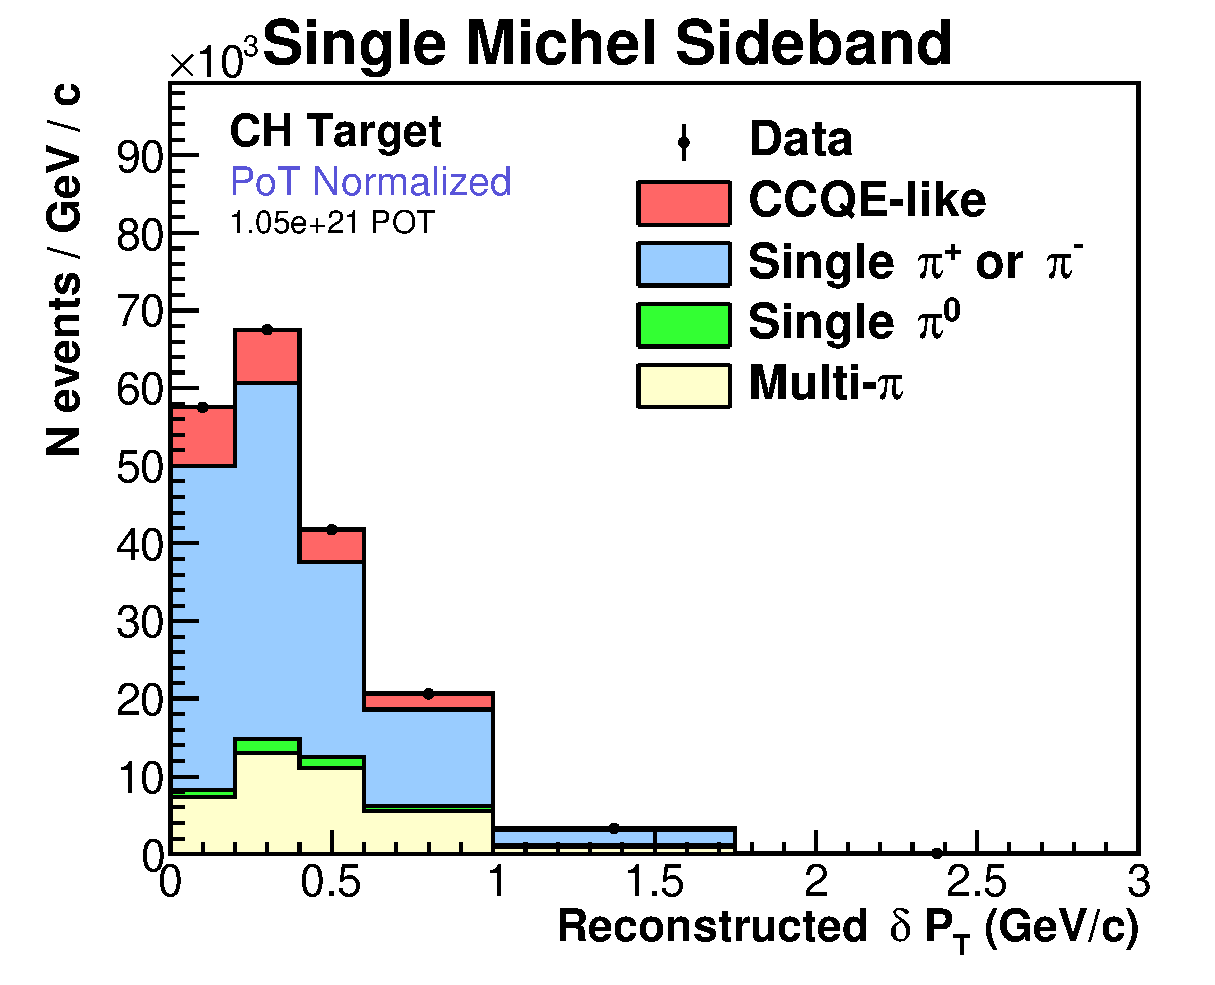
\includegraphics[width=0.48\linewidth]
{Figures/Sidebands/After/ch_sideband_michel_v5.eps}
 	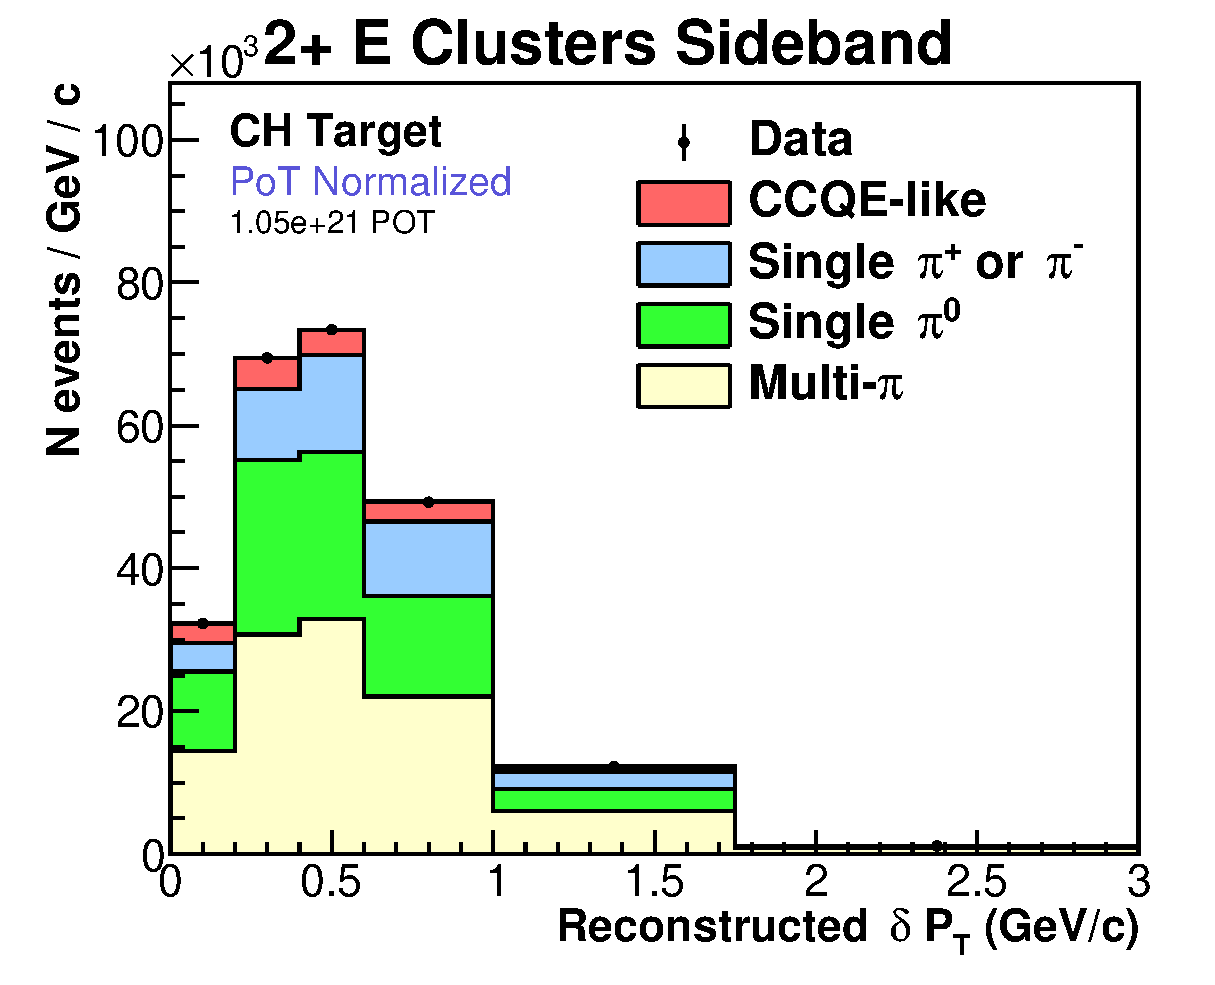
\includegraphics[width=0.48\linewidth]
{Figures/Sidebands/After/ch_sideband_energy_clusters_v5.eps}
	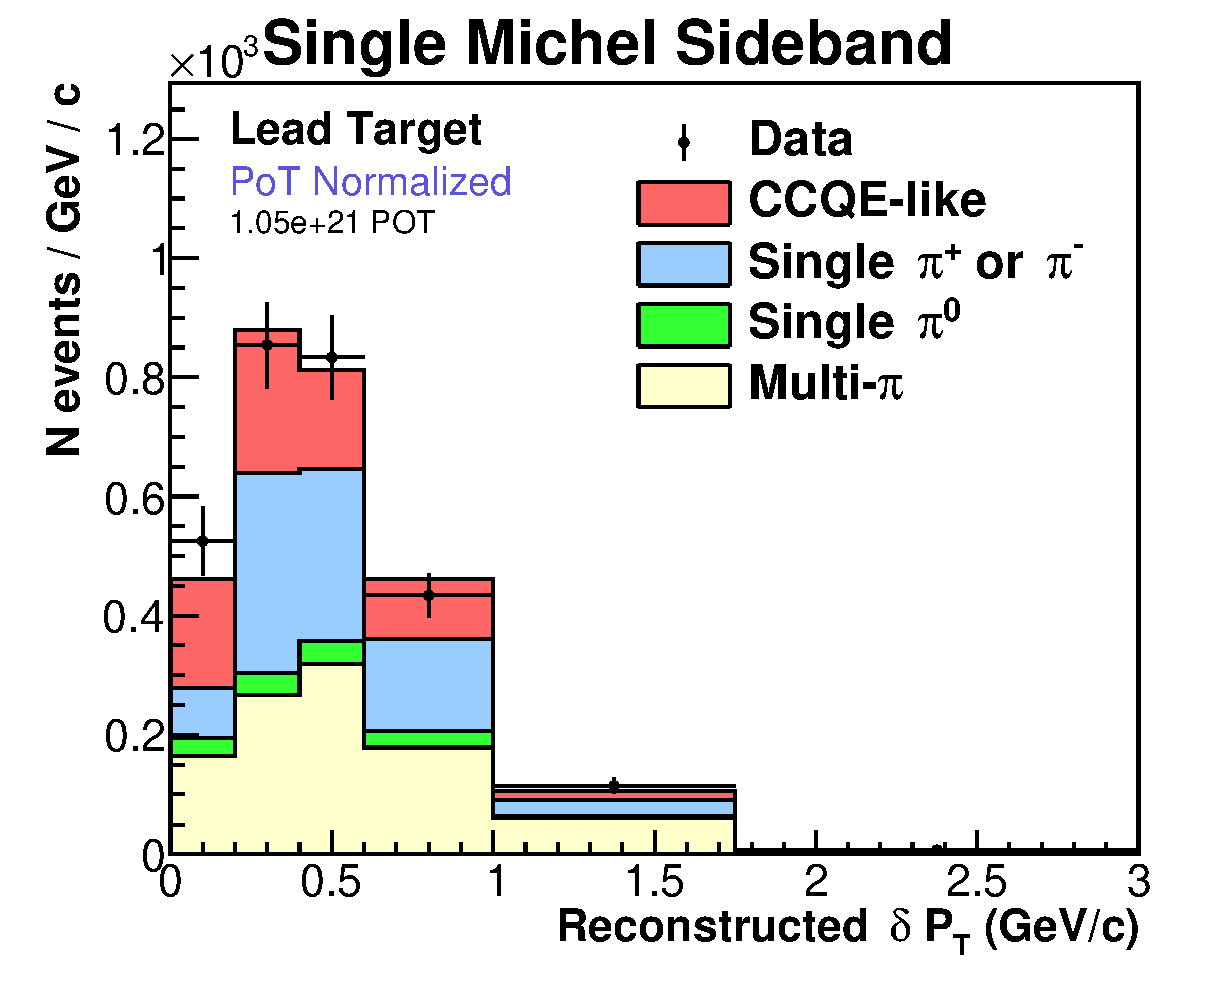
\includegraphics[width=0.48\linewidth]
{Figures/Sidebands/After/lead_sideband_michel_v5.eps}
 	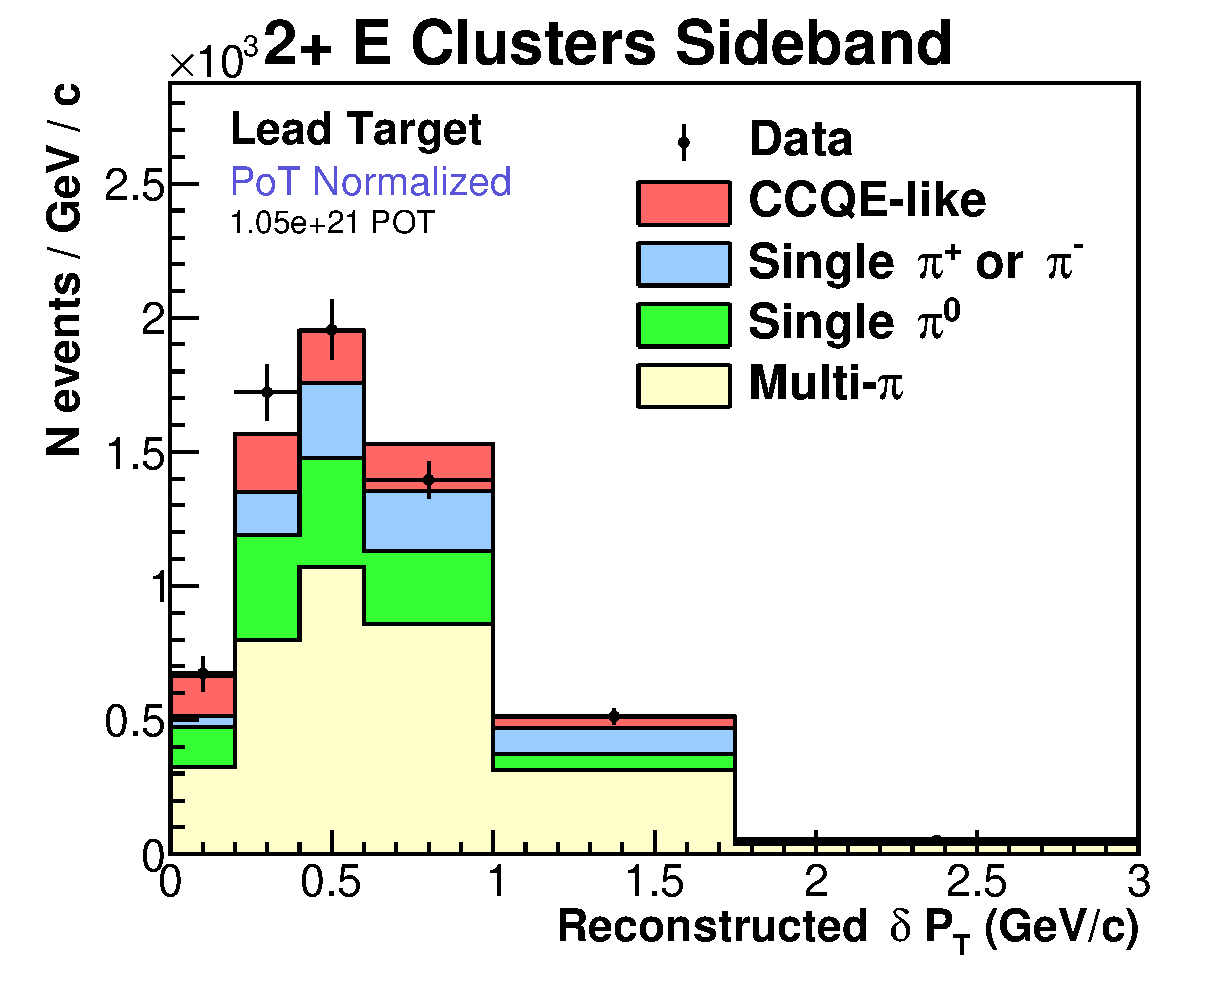
\includegraphics[width=0.48\linewidth]
{Figures/Sidebands/After/lead_sideband_energy_clusters_v5.eps}
	\caption{Event rates as a function of \tkidelta\ for the two sideband samples for scintillator (CH) and lead targets after background tuning. }
	\label{fig:tkidelta_sdbn_evntrate_tuned}
\end{figure}

Figure~\ref{fig:tkidelta_evntrate_tuned} shows the event rate in the signal region after tuning for each target except carbon, before background subtraction.  The predicted contributions from each background after tuning are also shown. 

 %\pagebreak



% tki_muon_pt event rate before background subtraction
\begin{figure}[h!]
	\centering
	\includegraphics[width=0.49\linewidth]%
{Figures/Supp_Events/ch_signal_after.eps}
\includegraphics[width=0.49\linewidth]%
{Figures/Supp_Events/h2o_signal_after.eps}
\includegraphics[width=0.49\linewidth]%
{Figures/Supp_Events/iron_signal_after.eps}
\includegraphics[width=0.49\linewidth]%
{Figures/Supp_Events/lead_signal_after.eps}
	\caption{Signal sample event rates as a function of \tkidelta \ for CH, C, H$_{2}$O, Fe, and Pb targets after background tuning but before background subtraction.}
	\label{fig:tkidelta_evntrate_tuned}
\end{figure}
%\FloatBarrier
Figure~\ref{fig:tkidelta_evntrate_backgroundsubtr} shows the signal for each target as a function of \tkiptmu\ after the backgrounds are subtracted.  In this procedure, the background removed is that predicted in the simulation after the background tuning.  The figure shows the various signal contributions to the quasielastic-like interaction.  Note that the quasielastic contribution to quasielastic-like events are predicted to be the most important at low \tkidelta\ but are only a small fraction of the event rate at high \tkidelta .  

% tki_muon_pt event rate after background subtraction
\begin{figure}[h!] 
	\centering
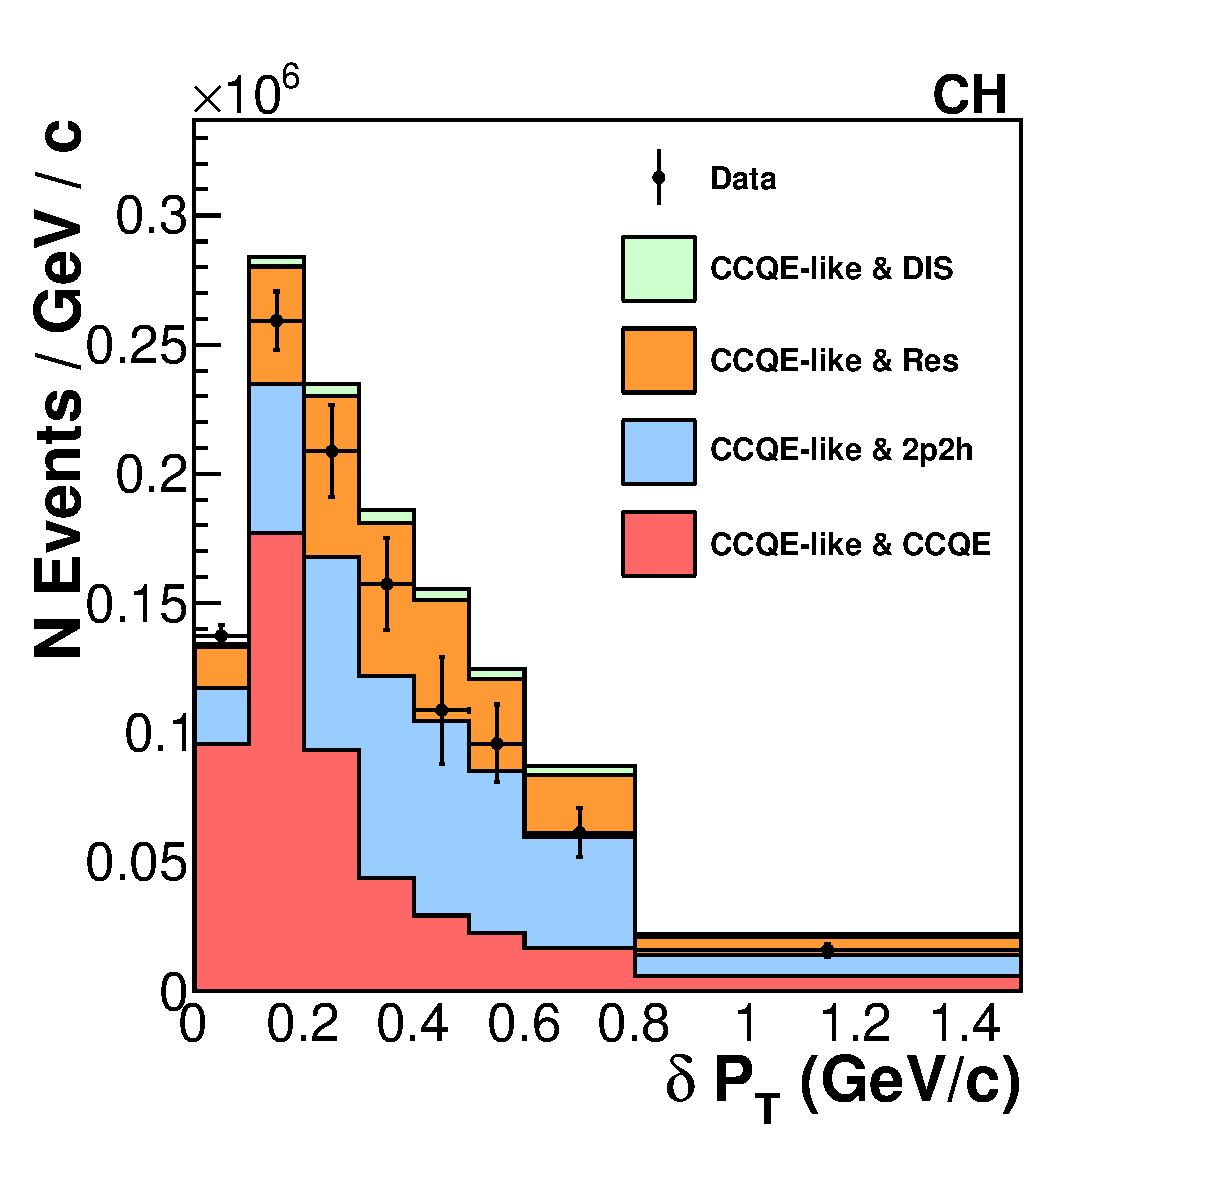
\includegraphics[width=0.49\linewidth]
{Figures/Supp_Events/background_subtracted_tki_dpt_fine_tracker.eps}	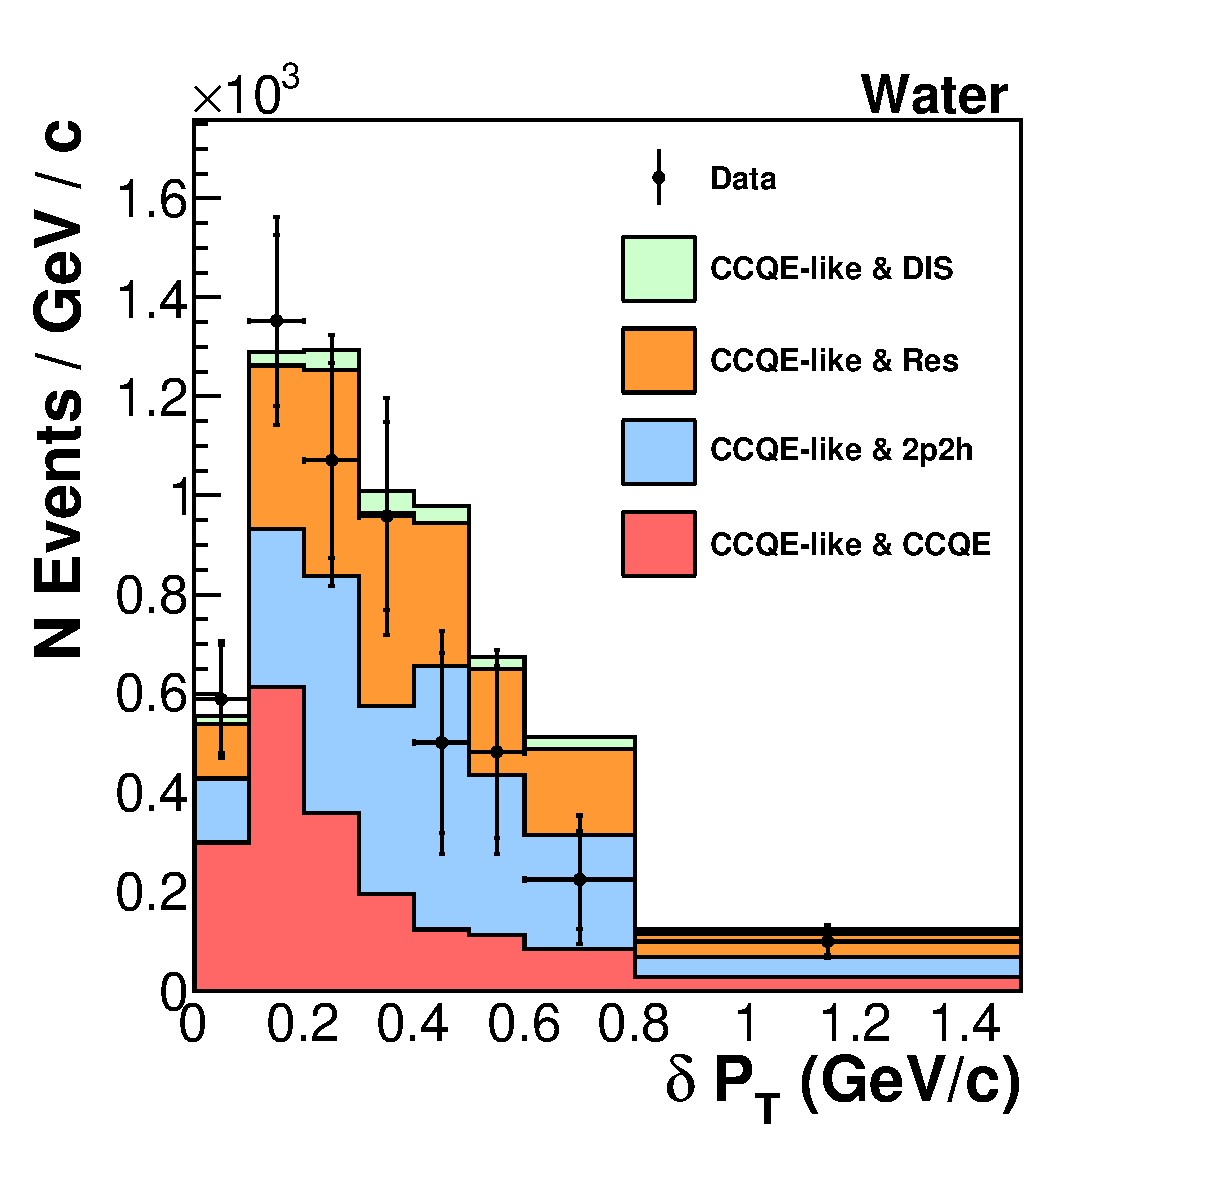
\includegraphics[width=0.49\linewidth]
{Figures/Supp_Events/background_subtracted_tki_dpt_fine_water.eps}
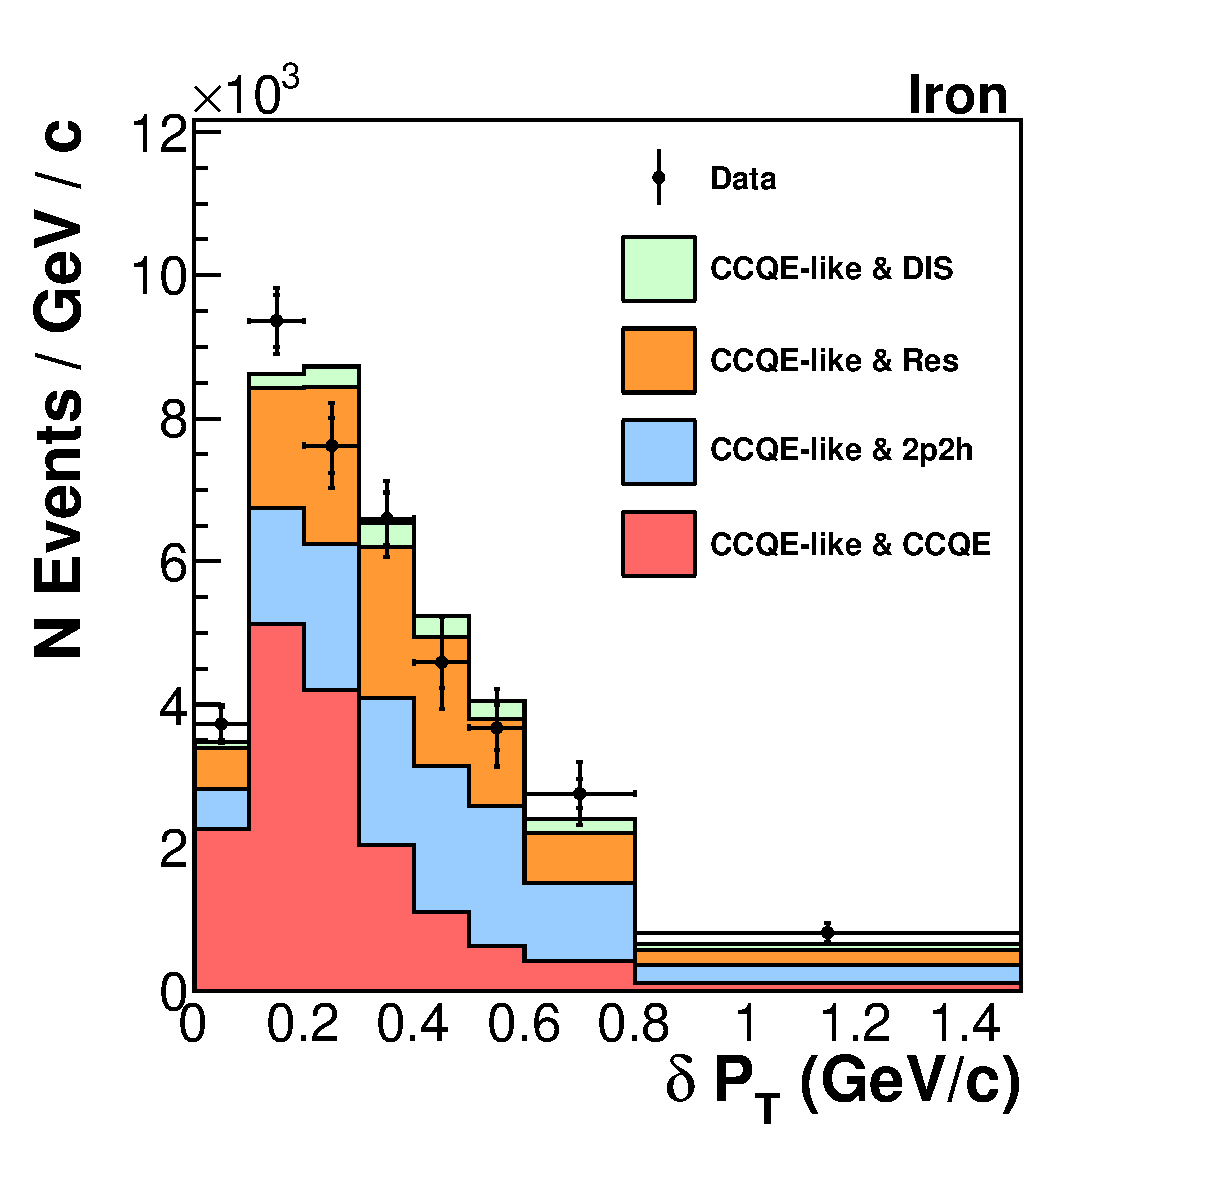
\includegraphics[width=0.49\linewidth]
{Figures/Supp_Events/background_subtracted_tki_dpt_fine_iron.eps}
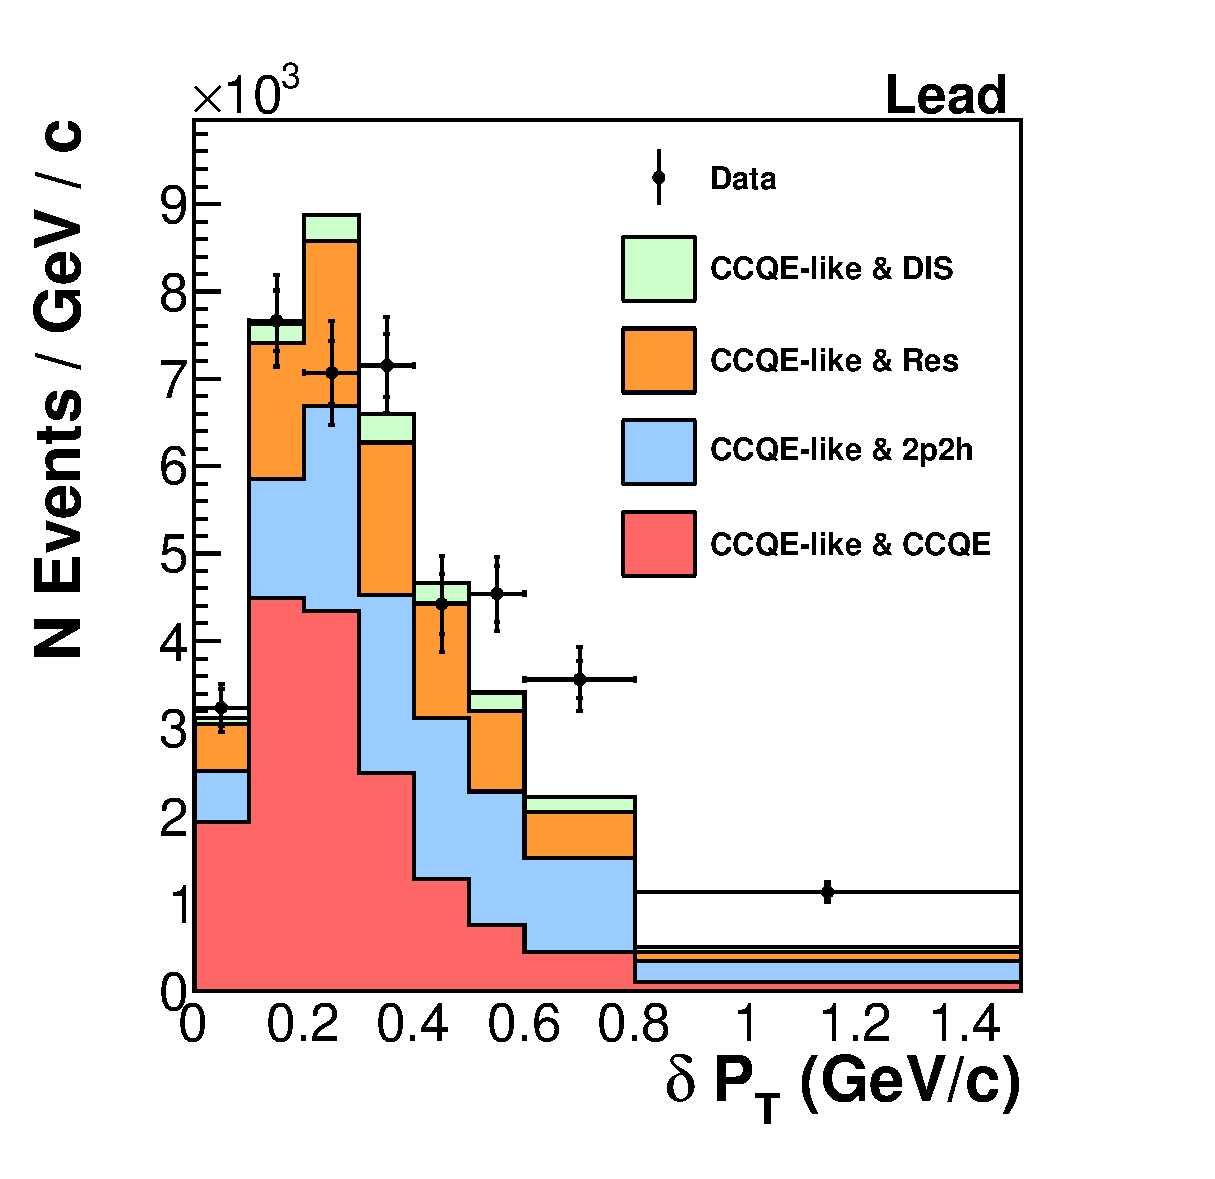
\includegraphics[width=0.49\linewidth]
{Figures/Supp_Events/background_subtracted_tki_dpt_fine_lead.eps}
	\caption{Signal sample event rates as a function of \tkidelta \ for CH, C, H$_{2}$O, Fe, and Pb targets after the tuned background has been subtracted.}
\label{fig:tkidelta_evntrate_backgroundsubtr}
\end{figure}

Once the backgrounds have been subtracted, the remaining event distributions can be unfolded as described in section~\ref{sec:analysis}.  The unfolded \tkidelta \ event rate distributions for water, iron, lead and scintillator are shown in Fig.~\ref{fig:tkidelta_evntrate_unfolded}.  

% tki_muon_pt event rate after unfolding
\begin{figure}  
	\centering
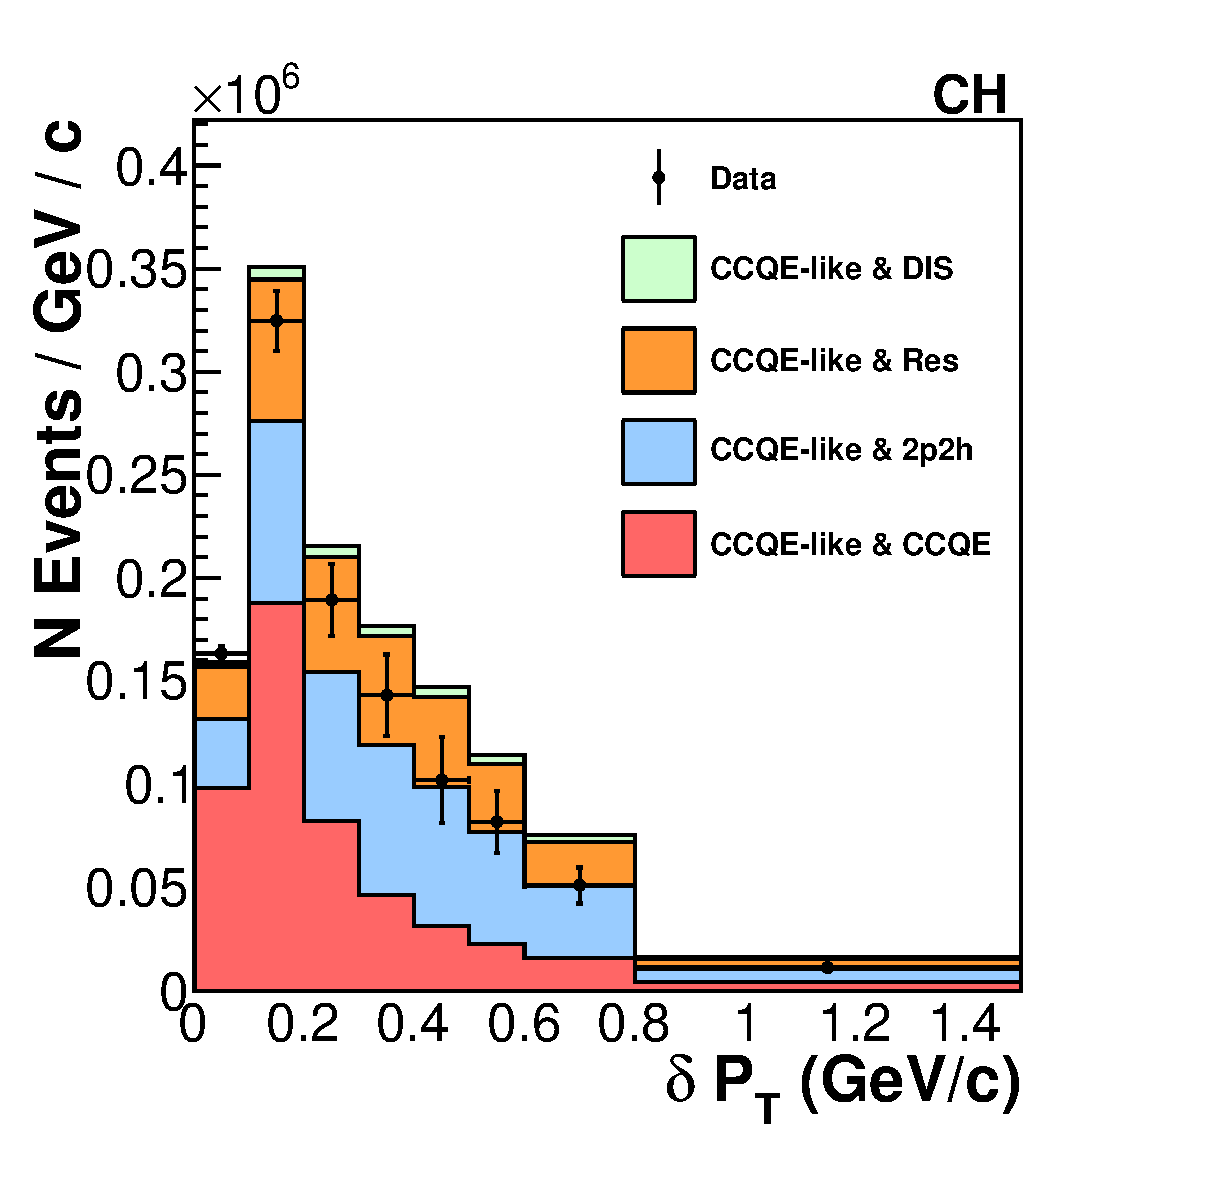
\includegraphics[width=0.49\linewidth] {Figures/Supp_Events/unfolded_tki_dpt_fine_tracker.eps}
  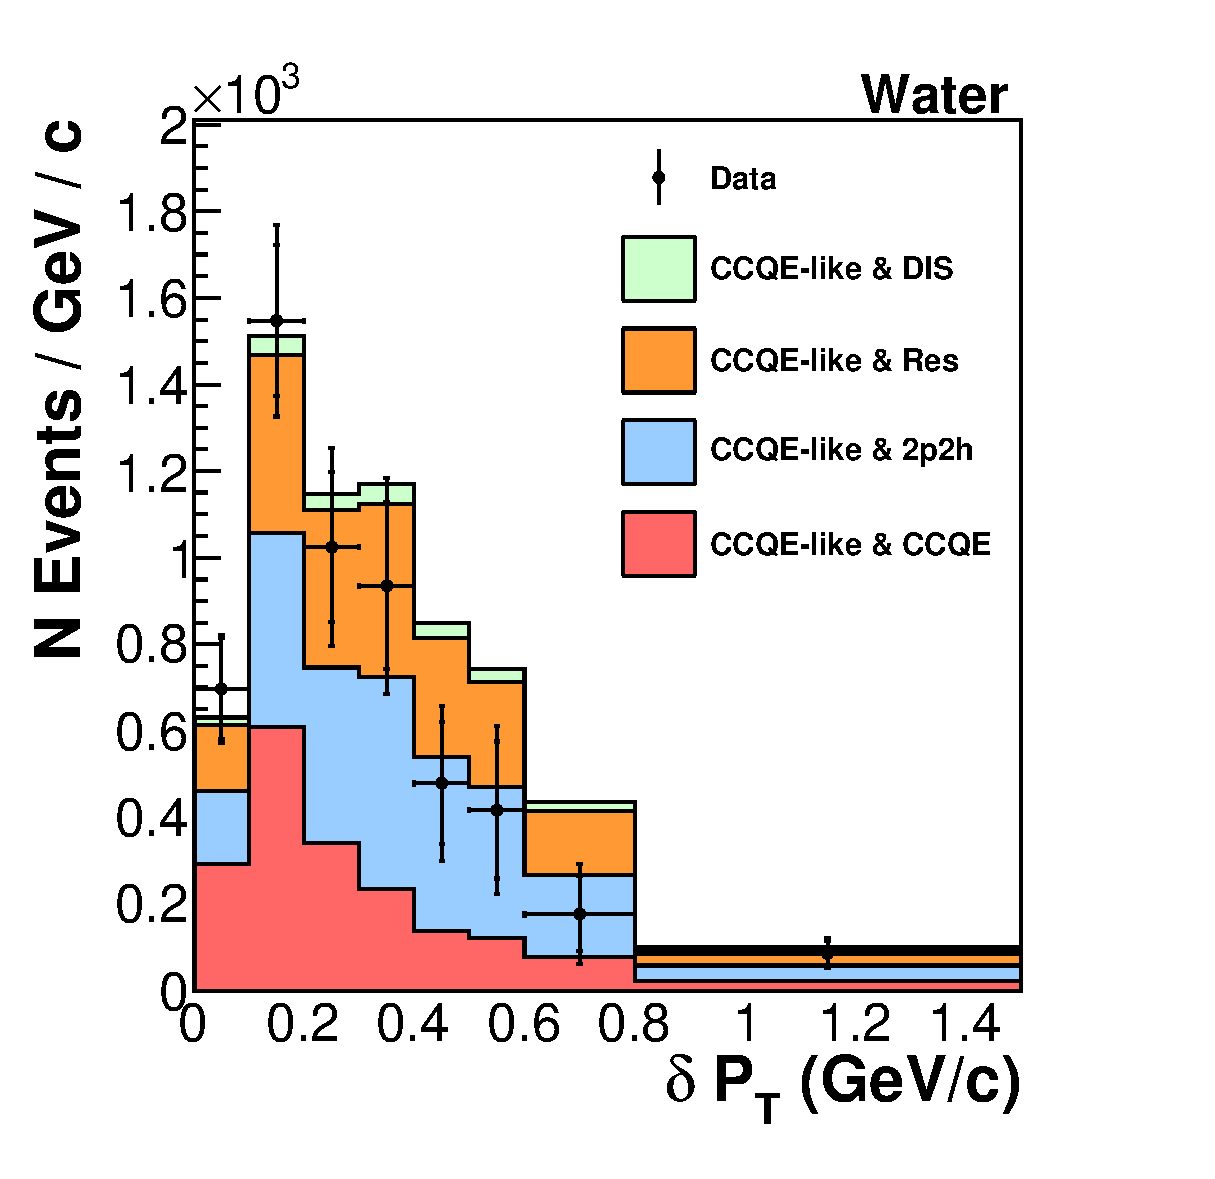
\includegraphics[width=0.49\linewidth]
{Figures/Supp_Events/unfolded_tki_dpt_fine_water.eps}
   	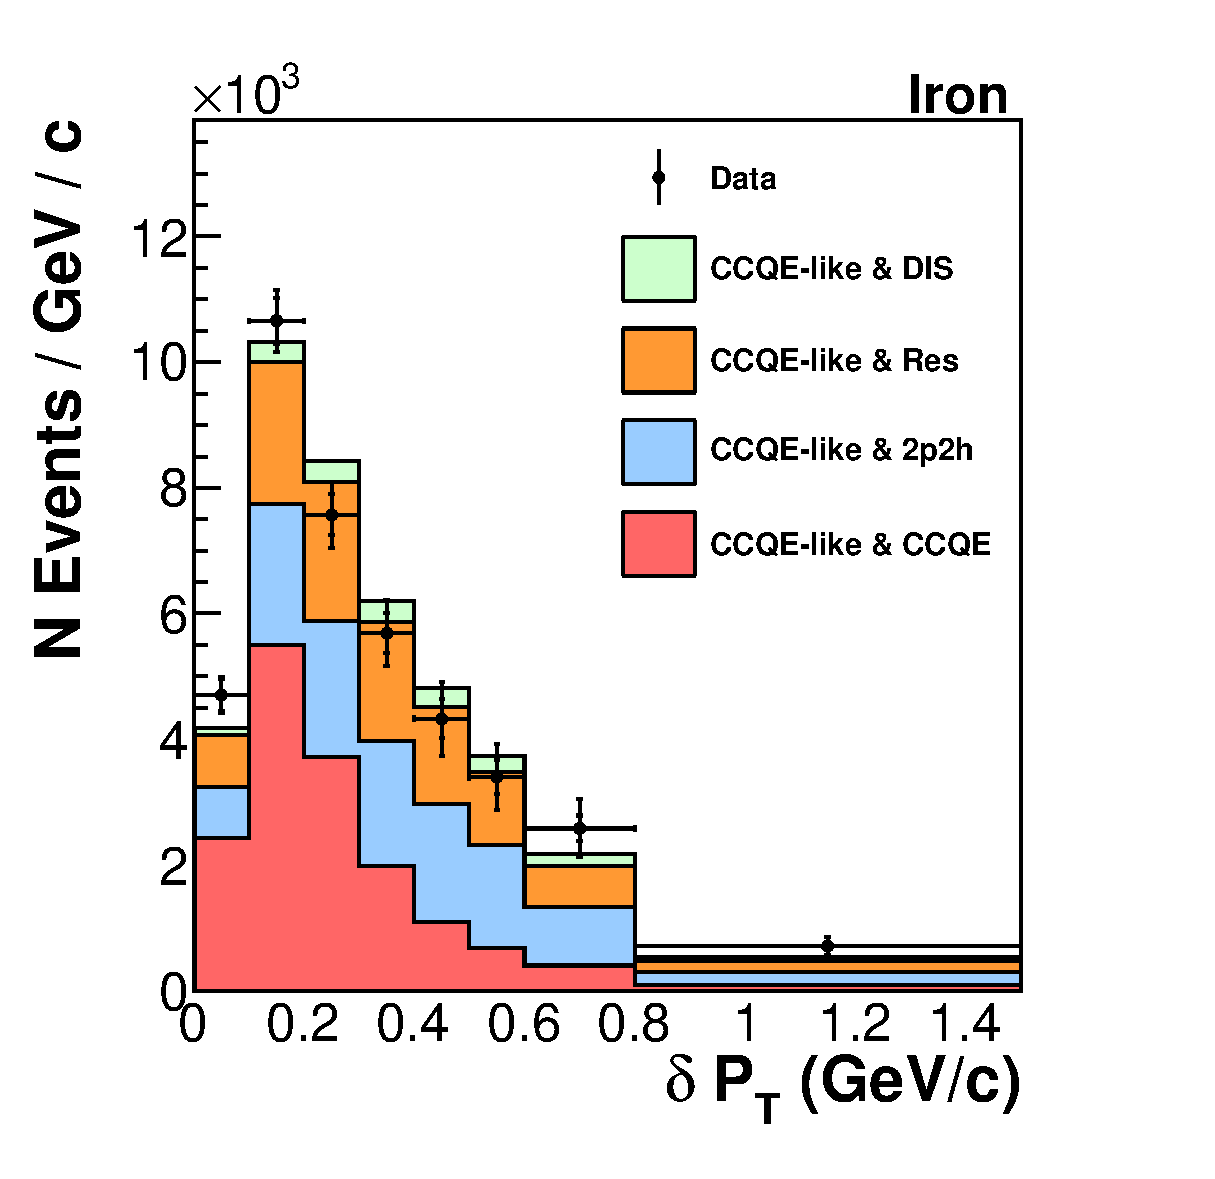
\includegraphics[width=0.49\linewidth]
{Figures/Supp_Events/unfolded_tki_dpt_fine_iron.eps}
    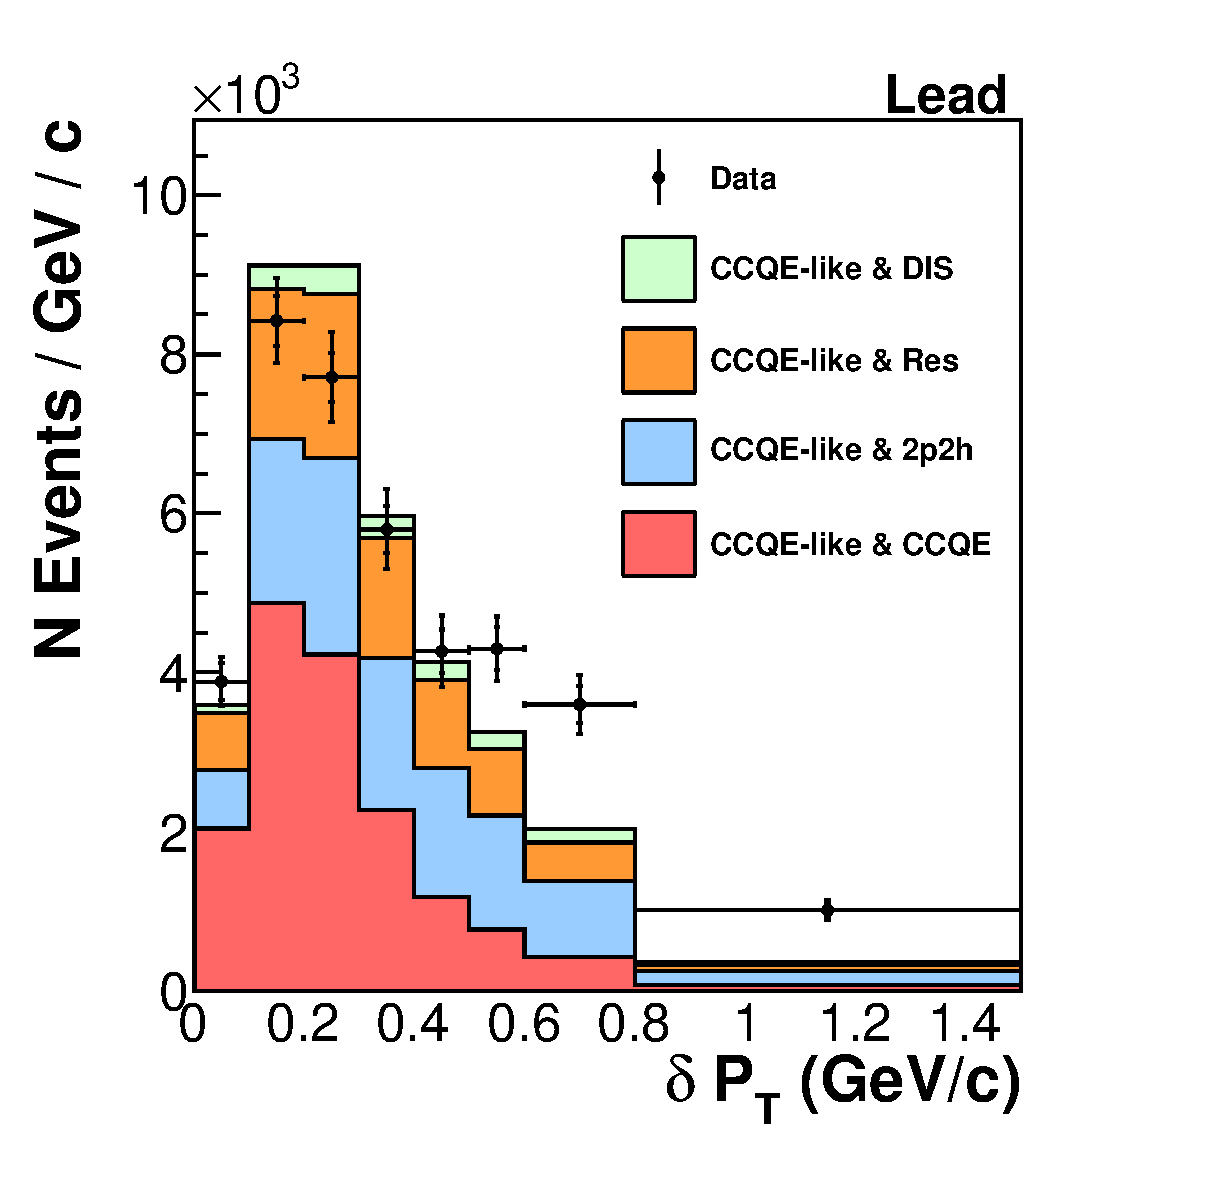
\includegraphics[width=0.49\linewidth]
{Figures/Supp_Events/unfolded_tki_dpt_fine_lead.eps}
	\caption{Signal sample event rates as a function of \tkidelta \ for CH, C, H$_{2}$O, Fe, and Pb targets after unfolding. }
	\label{fig:tkidelta_evntrate_unfolded}
\end{figure}

After the distributions have been unfolded, then the analysis divides by the efficiency as a function of \tkidelta\ for each target separately in the detector. 
 Figure~\ref{fig:tkidelta_efficiency} shows the average efficiency as function of \tkidelta \ for scintillator on the left and for lead on the right. 

% tkidelta efficiency correction for CH and Pb
\begin{figure}[h]
	\centering
	\includegraphics[width=.48\linewidth]%{Figures/TKI_muon_pt/tracker_eff_muon_pt.eps}
 {Figures/Event_rate_plots/TKIdelta/reco_eff/tracker_v5.eps}
 	\includegraphics[width=.48\linewidth]%{Figures/TKI_muon_pt/lead_eff_muon_pt.eps}
   {Figures/Event_rate_plots/TKIdelta/reco_eff/lead_v5.eps}
	\caption{The signal efficiency as  a function of \tkidelta\ for events from interactions on CH on the left and Pb on the right.}
	\label{fig:tkidelta_efficiency}
\end{figure}

As described in Sec.\ref{sec:analysis}, the flux varies somewhat across the face of the detector.  The variations for each individual target are accounted for in the analysis, and the average variation of the flux for each nuclear target type is shown in Fig.~\ref{fig:fluxes}.  Because the lead targets are distributed in locations that are appoximately symmetric around the center of the detector, the net effect for lead is small.  Similarly, the water target itself is also symmetric around the center of the detector so there is no correction needed for the water to scintillator comparisons.  
\begin{figure}[tb]
\centering
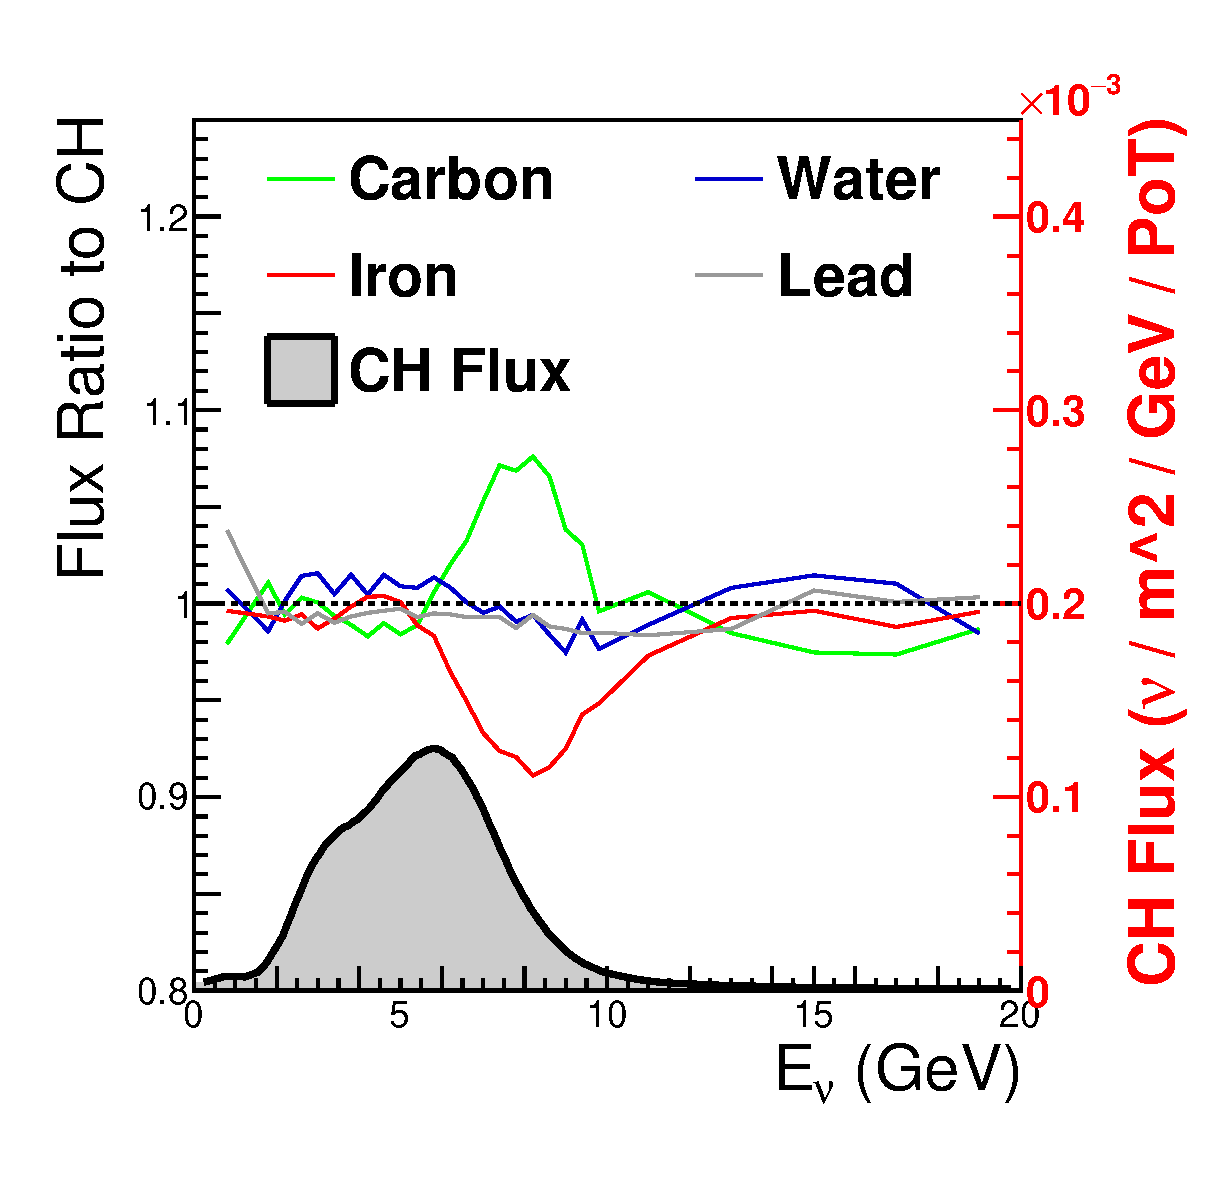
\includegraphics[width=\linewidth]{Figures/fluxes.eps}
\caption{The ratio of the flux in each target material to that in the scintillator target.}
\label{fig:fluxes}
\end{figure}

\clearpage
\subsection{Supplemental:  Cross-section Ratios to GENIE}
\label{sec:appendixA}
Ratios between the data and the default tuned GENIE simulation are shown in the plots in this section.  The ratios between the various model choices in different generators and the default tuned GENIE simulation are also shown in this section.  The descriptions of the different model choices for each generator are described in Tab.~\ref{tab:generators}.  In many kinematic regions the measurement uncertainties are considerably smaller than the variations between different models, especially for the heavier nuclear targets and for scintillator where the statistics are the highest.  
\begin{figure}
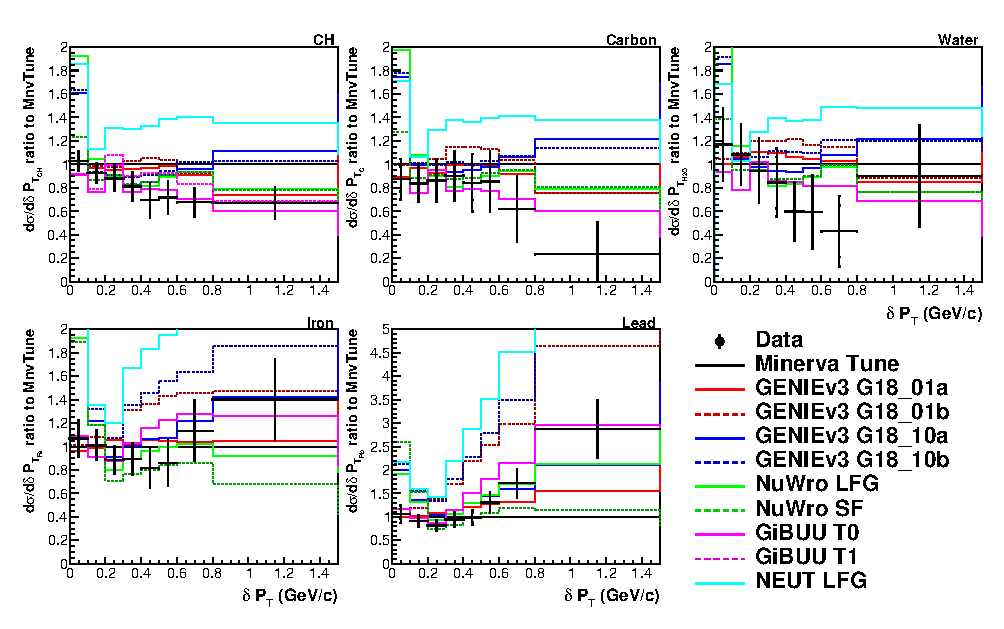
\includegraphics[width=\linewidth]{Figures/gencompare_ratio/mnvratio_dpt_fine.eps}
    \caption[\tkidelta \ cross-section comparison to the MINERvA tune for multiple targets ]{Ratio of absolute cross section measurements to the MINERvA tune for different targets as a function of \tkidelta\ and ratios of different model predictions to the MINERvA tune. 
    }
    \label{fig:models_dpt_rat}
\end{figure}
\begin{figure}
    \centering
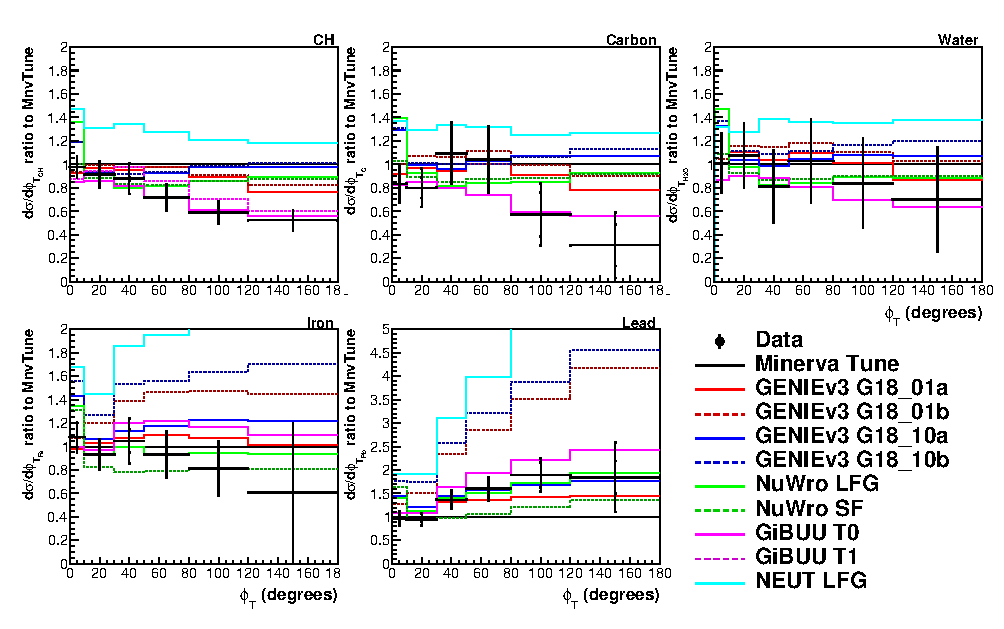
\includegraphics[width=\linewidth]{Figures/gencompare_ratio/mnvratio_phi.eps}
    \caption[\tkicoplanar \ cross-section ratio to the MINERvA tune for multiple targets ]{Ratio of absolute cross section measurements to the MINERvA tune for different targets as a function of  \tkicoplanar\ and ratios of different model predictions to the MINERvA tune.}
    \label{fig:models_coplan_rat}
\end{figure}
\begin{figure}
    \centering
    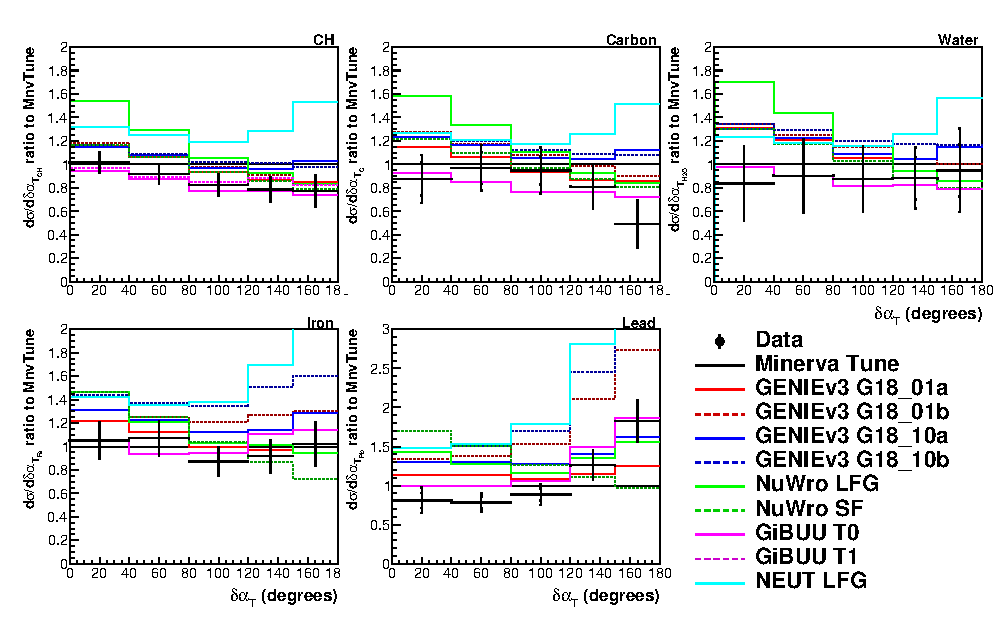
\includegraphics[width=\linewidth]{Figures/gencompare_ratio/mnvratio_alpha.eps}
    \caption[\tkialpha \ cross-section comparison for multiple targets ]{Ratio of absolute cross section measurements to the MINERvA tune for different targets as a function of  \tkialpha\ and ratios of different model predictions to the MINERvA tune.}
    \label{fig:models_alphat_rat}
\end{figure}
\begin{figure}
    \centering
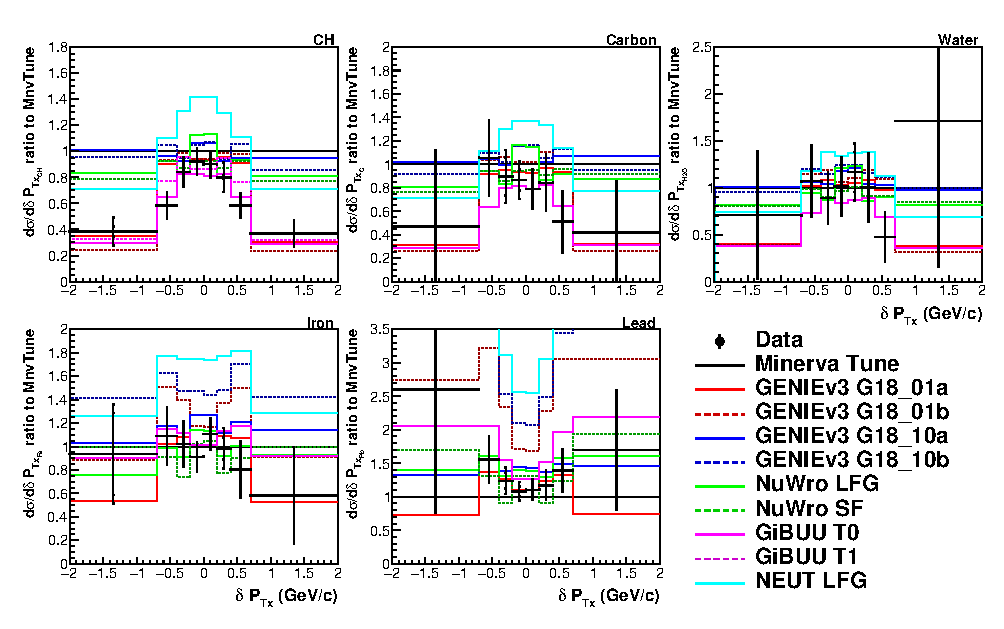
\includegraphics[width=\linewidth]{Figures/gencompare_ratio/mnvratio_dptx.eps}
    \caption{Ratio of absolute cross section measurements to the MINERvA tune for different targets as a function of  \tkidptx\ and ratios of different model predictions to the MINERvA tune.}
    \label{fig:models_dptx_rat}
\end{figure}
\begin{figure}
    \centering
    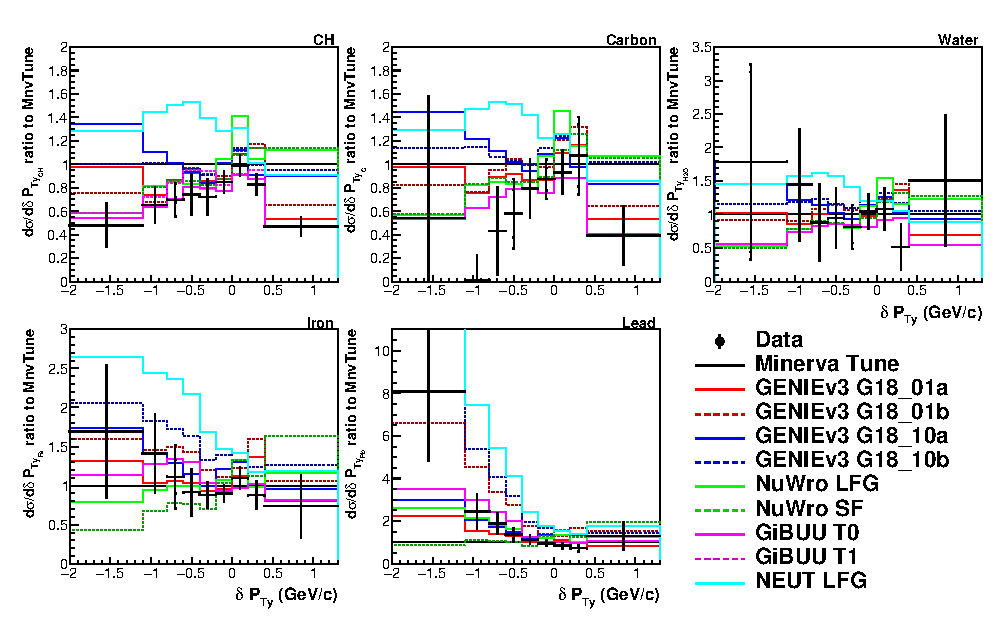
\includegraphics[width=\linewidth]{Figures/gencompare_ratio/mnvratio_dpty.eps}
     \caption{Ratio of absolute cross section measurements to the MINERvA tune for different targets as a function of  \tkidpty\ and ratios of different model predictions to the MINERvA tune. }
    \label{fig:models_dpty_rat}
\end{figure}
\begin{figure}
    \centering
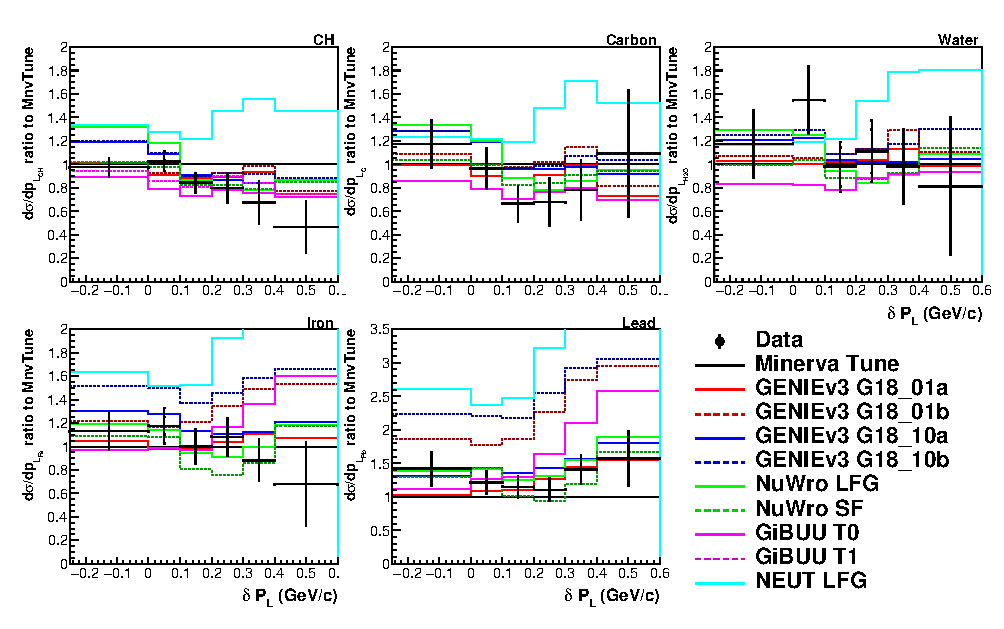
\includegraphics[width=\linewidth]{Figures/gencompare_ratio/mnvratio_pl.eps}
    \caption{Ratio of absolute cross section measurements to the MINERvA tune for different targets as a function of  \tkipl\ and ratios of different model predictions to the MINERvA tune.}
    \label{fig:models_pl_rat}
\end{figure}
\begin{figure}
    \centering            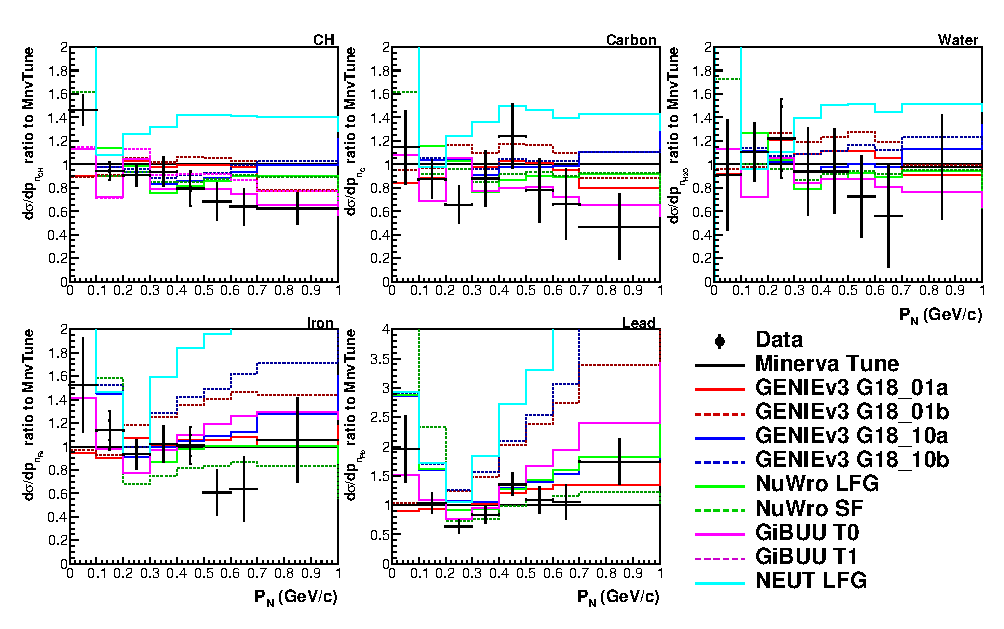
\includegraphics[width=\linewidth]{Figures/gencompare_ratio/mnvratio_pn.eps}
    \caption{Ratio of absolute cross section measurements to the MINERvA tune for different targets as a function of  \tkipn\ and ratios of different model predictions to the MINERvA tune.}
    \label{fig:models_pn_rat}
\end{figure}
\begin{figure}
    \centering
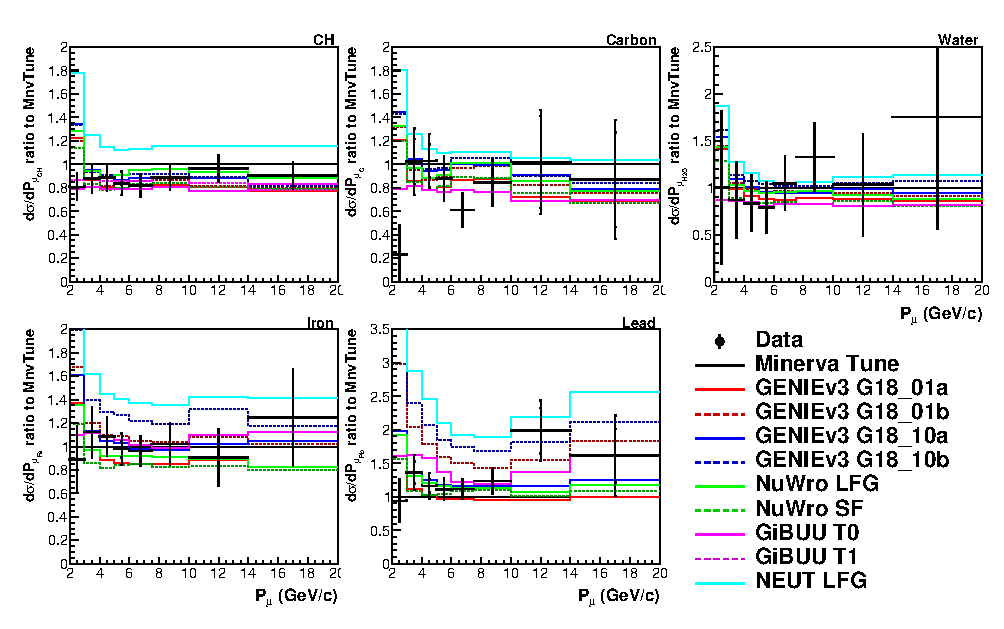
\includegraphics[width=\linewidth]{Figures/gencompare_ratio/mnvratio_muon_p.eps}
    \caption{Ratio of absolute cross section measurements to the MINERvA tune for different targets as a function of  P$_\mu$ and ratios of different model predictions to the MINERvA tune.}
    \label{fig:models_muon_p_rat}
\end{figure}
\begin{figure}
    \centering
    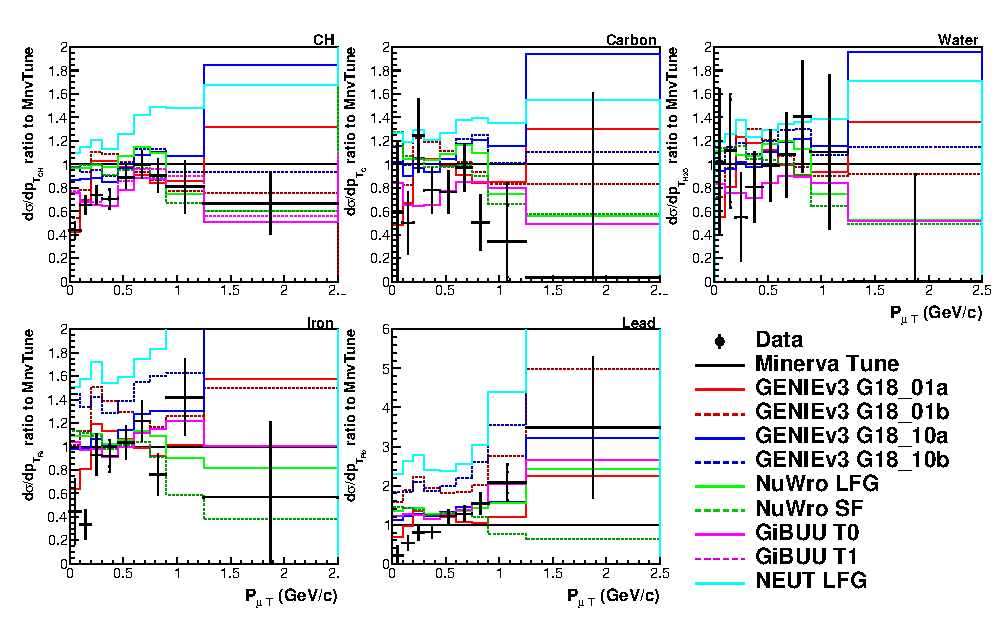
\includegraphics[width=\linewidth]{Figures/gencompare_ratio/mnvratio_muon_pt.eps}
    \caption[\tkiptmu \ cross-section comparison for multiple targets ]{Ratio of absolute cross section measurements to the MINERvA tune for different targets as a function of  \tkiptmu\ and ratios of different model predictions to the MINERvA tune.}
    \label{Figure:Gencompare_ptmu_rat}
\end{figure}
\begin{figure}
    \centering
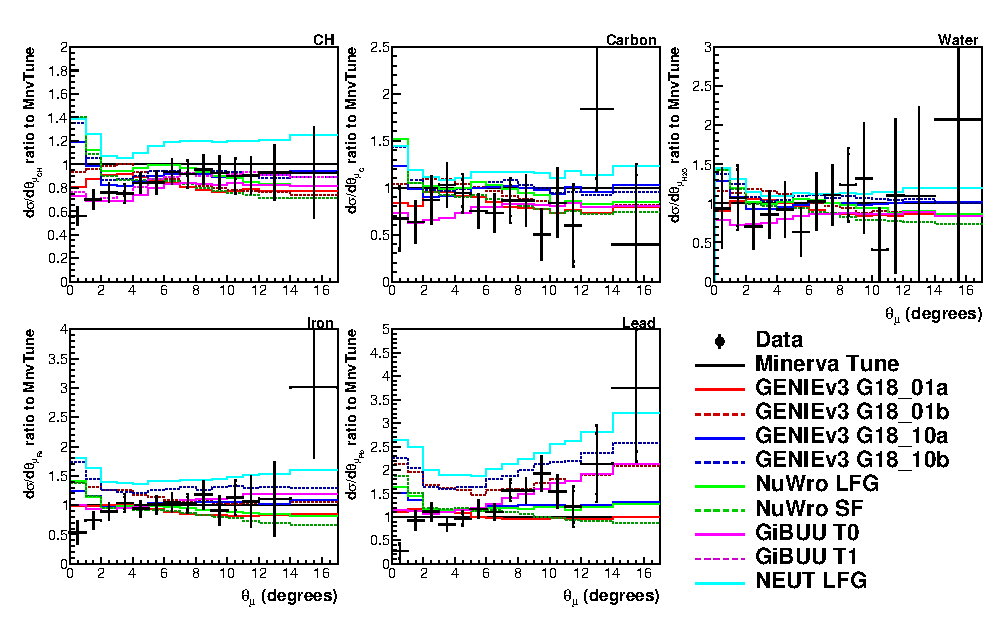
\includegraphics[width=\linewidth]{Figures/gencompare_ratio/mnvratio_muon_theta.eps}
    \caption{Ratio of absolute cross section measurements to the MINERvA tune for different targets as a function of $\theta_{\mu}$ and ratios of different model predictions to the MINERvA tune.}
    \label{fig:models_muon_theta_rat}
\end{figure}
\begin{figure}
    \centering
 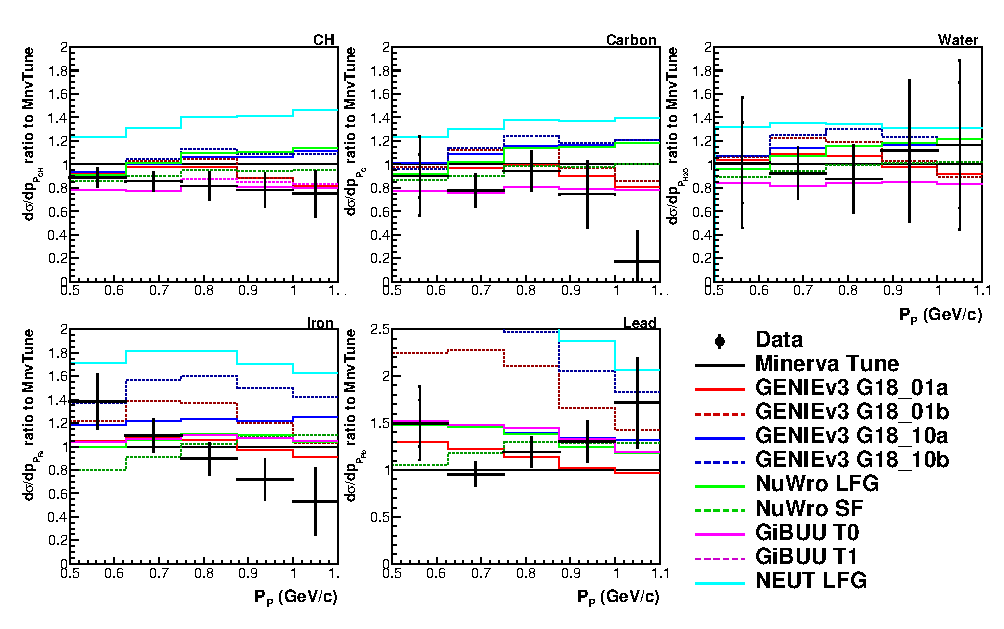
\includegraphics[width=\linewidth]{Figures/gencompare_ratio/mnvratio_proton_p.eps}
    \caption{Ratio of absolute cross section measurements to the MINERvA tune for different targets as a function of P$_{p}$ and ratios of different model predictions to the MINERvA tune.}
    \label{fig:models_proton_p_rat}
\end{figure}
\begin{figure}
    \centering
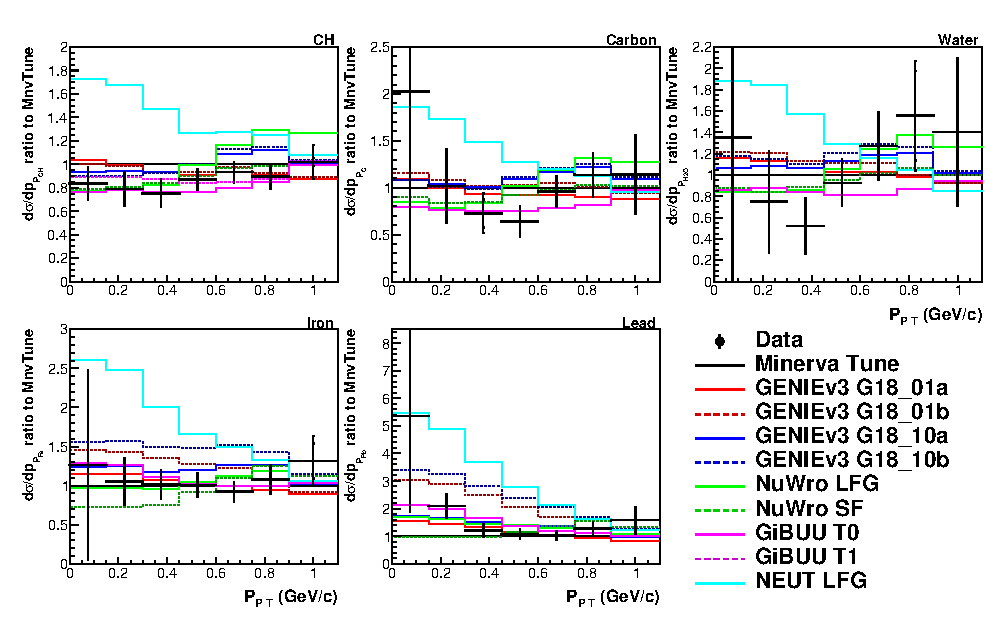
\includegraphics[width=\linewidth]{Figures/gencompare_ratio/mnvratio_proton_pt.eps}
    \caption{Ratio of absolute cross section measurements to the MINERvA tune for different targets as a function of P$_{p T}$ and ratios of different model predictions to the MINERvA tune.}
    \label{fig:models_proton_pt_rat}
\end{figure}
\begin{figure}
    \centering
    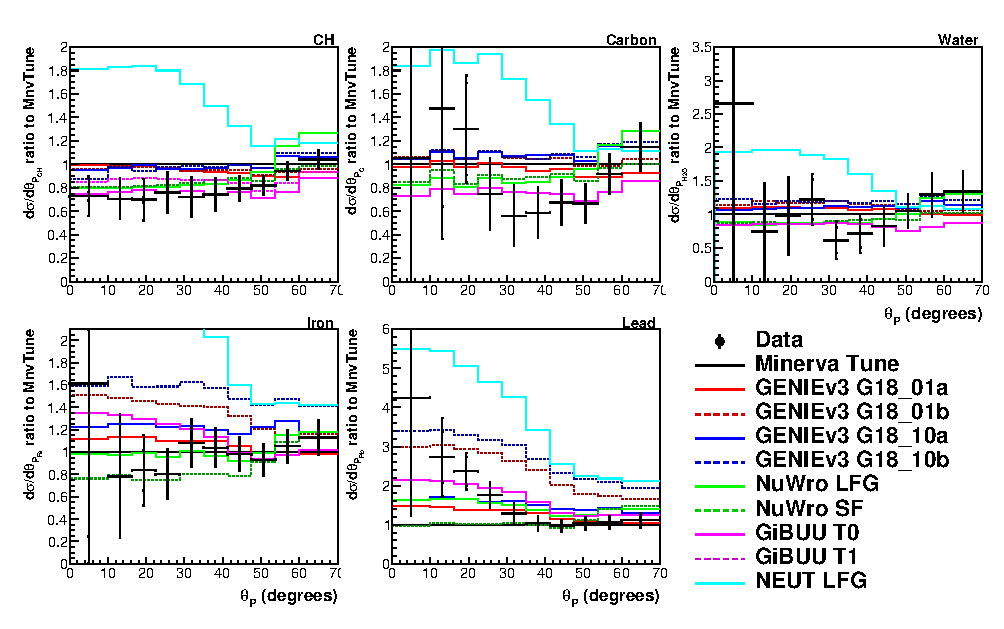
\includegraphics[width=\linewidth]{Figures/gencompare_ratio/mnvratio_proton_theta.eps}
    \caption{Ratio of absolute cross section measurements to the MINERvA tune for different targets as a function of $\theta_{p}$ and ratios of different model predictions to the MINERvA tune.}
    \label{fig:models_proton_theta_rat}
\end{figure}

\clearpage
% uncertainties in tki_coplanar xsecs
\subsection{Supplemental:  Uncertainties in Cross Sections and Ratios} 
\label{sec:appendixB}
The uncertainties on the absolute cross sections and cross-section ratios to scintillator (CH) as a function of all the kinematic variables besides described in the main body of the paper (except \tkidelta\ ) are presented in this Appendix.  The format for each figure is the same:  the top five plots show the uncertainties on the absolute cross sections for CH, carbon, water, iron and lead.  Note that because the statistical uncertainties in carbon and water are large compared to the other targets, those uncertainties have been scaled by 0.5 to be plotted next to the uncertainties on the CH target.  The bottom four plots show the uncertainties in the ratios of the absolute cross sections to CH.  Note that the flux and muon reconstruction uncertainties largely cancel in the ratio, and the statistical uncertainty in the ratio is close to that of the absolute cross sections due to the large mass of the scintillator (CH) target compared to the passive targets.  
\begin{figure}
	\centering
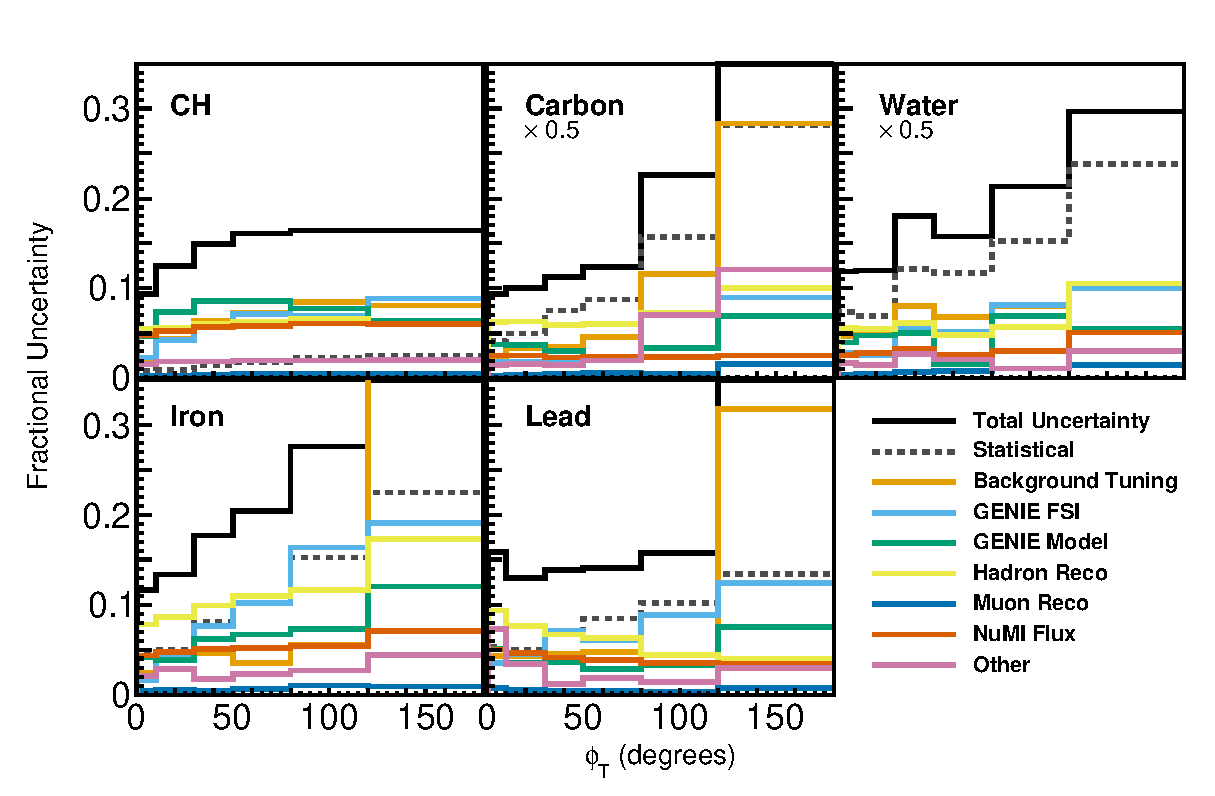
\includegraphics[width=\linewidth]{Figures/xsec_errors_all5/errors_phi.eps}
    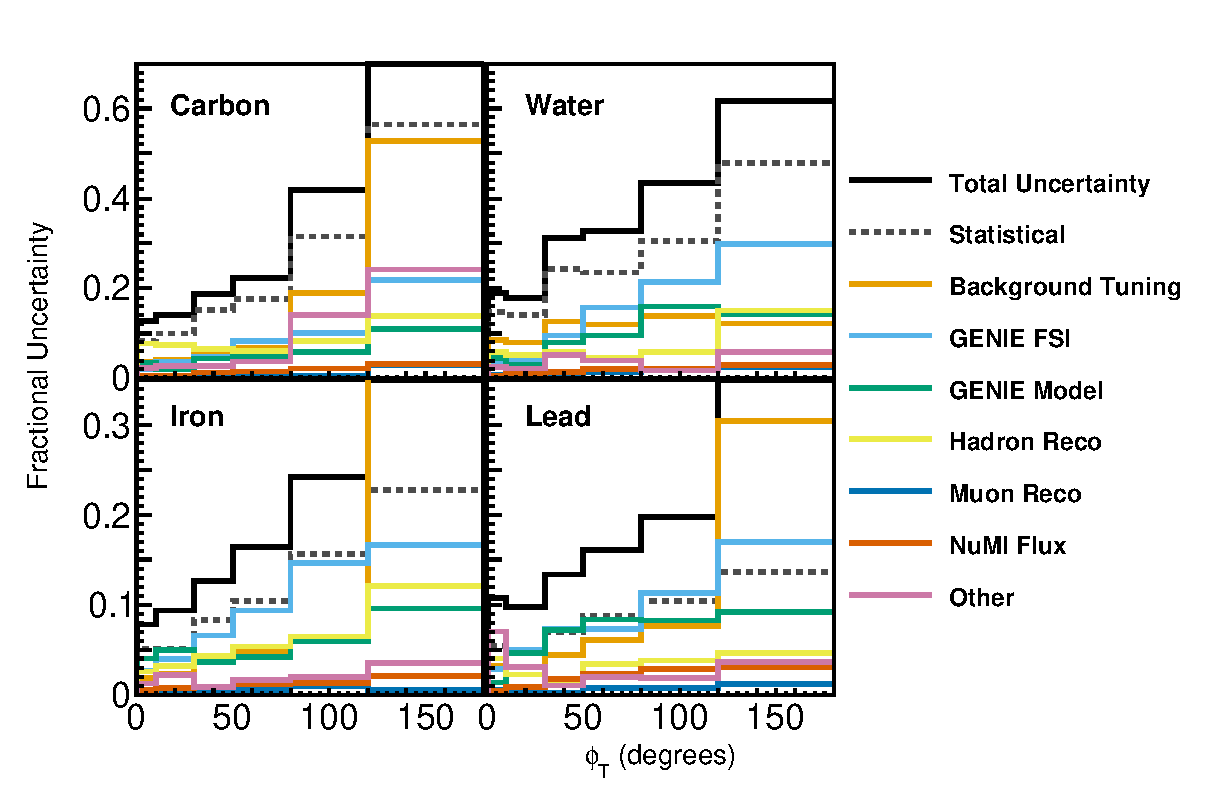
\includegraphics[width=\linewidth]{Figures/xsec_ratio_errors/ratio_errors_phi.eps}
    \caption[\tkicoplanar cross-section uncertainties for multiple targets]{Uncertainties on the absolute cross section for each target (upper five plots) and on the ratio to CH (lower four plots) for \tkicoplanar.}
    \label{fig:xsec_err_coplan}
\end{figure}
% uncertainties in tki_alpha xsecs
%
%  alpha
%
\begin{figure}
	\centering
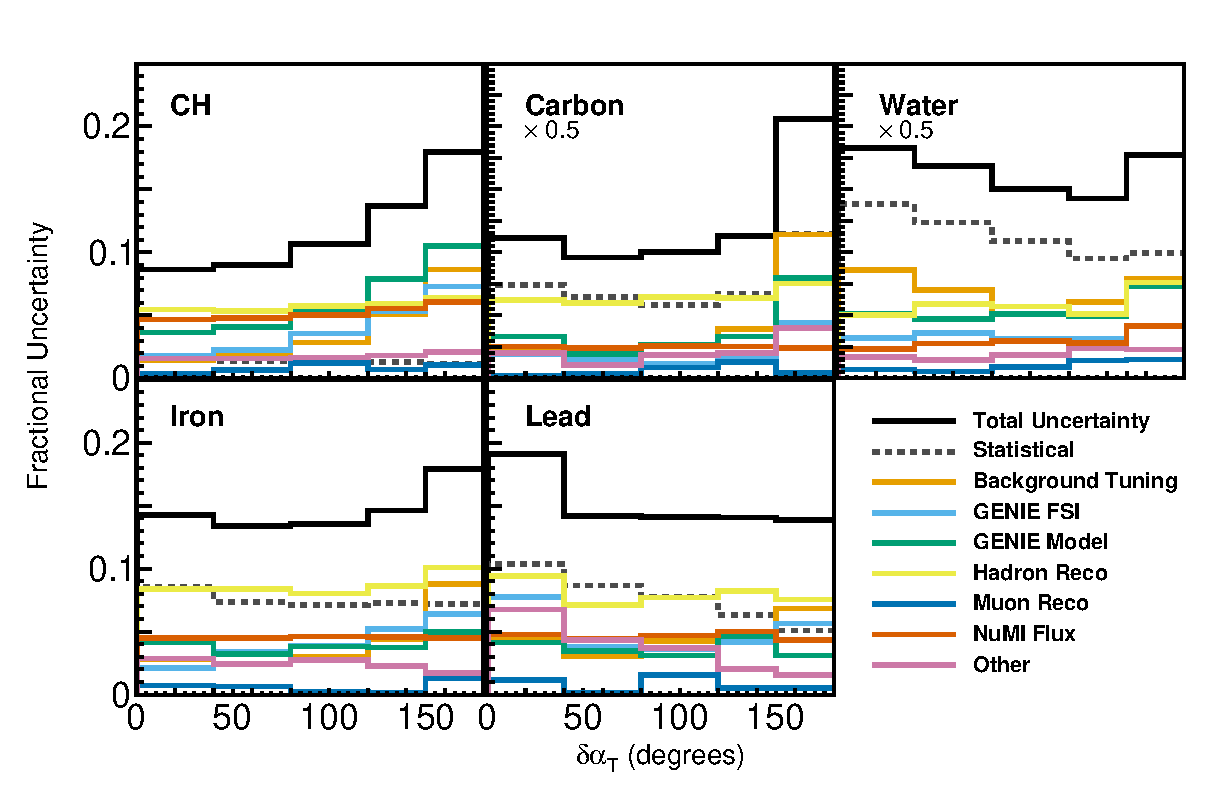
\includegraphics[width=\linewidth]{Figures/xsec_errors_all5/errors_alpha.eps}
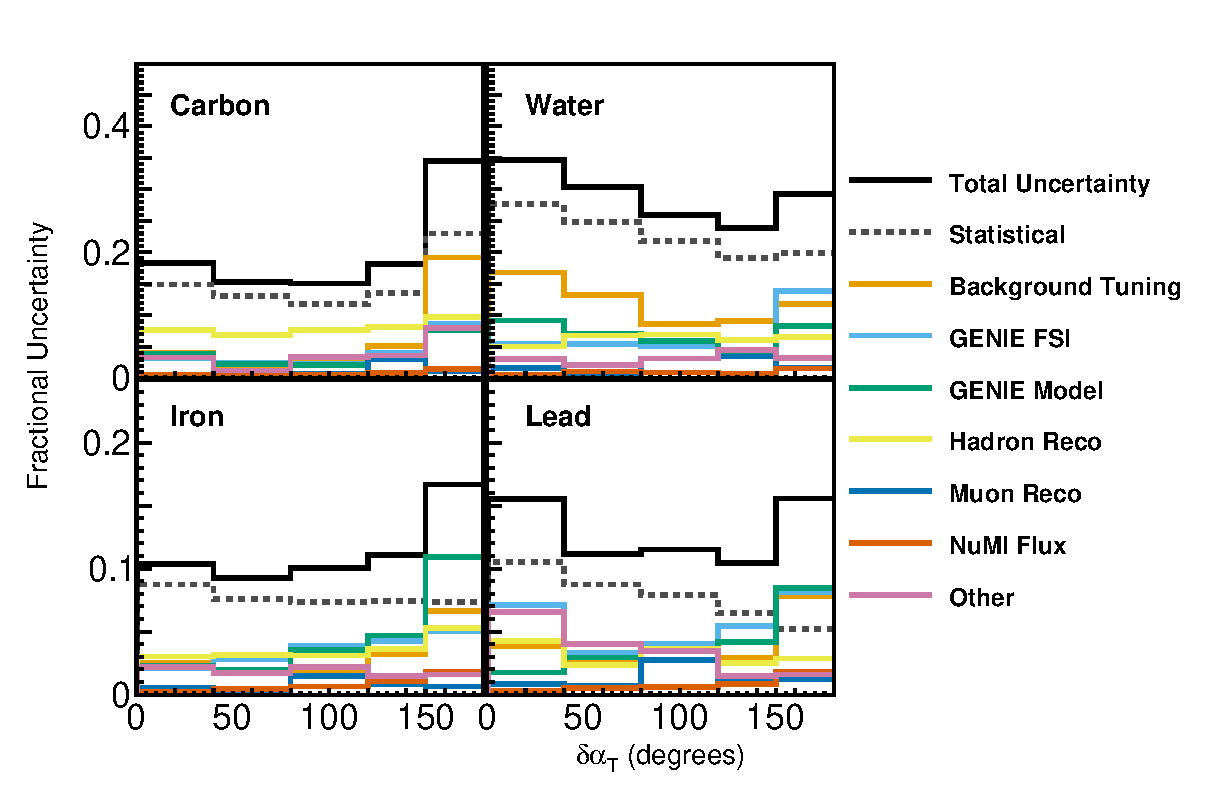
\includegraphics[width=\linewidth]{Figures/xsec_ratio_errors/ratio_errors_alpha.eps}
    \caption[\tkialpha cross-section uncertainties for multiple targets]{Uncertainties on the absolute cross section for each target (upper five plots) and on the ratio to CH (lower four plots) for \tkialpha.}
    \label{fig:xsec_err_alpha}
\end{figure}
% dptx
\begin{figure}
	\centering
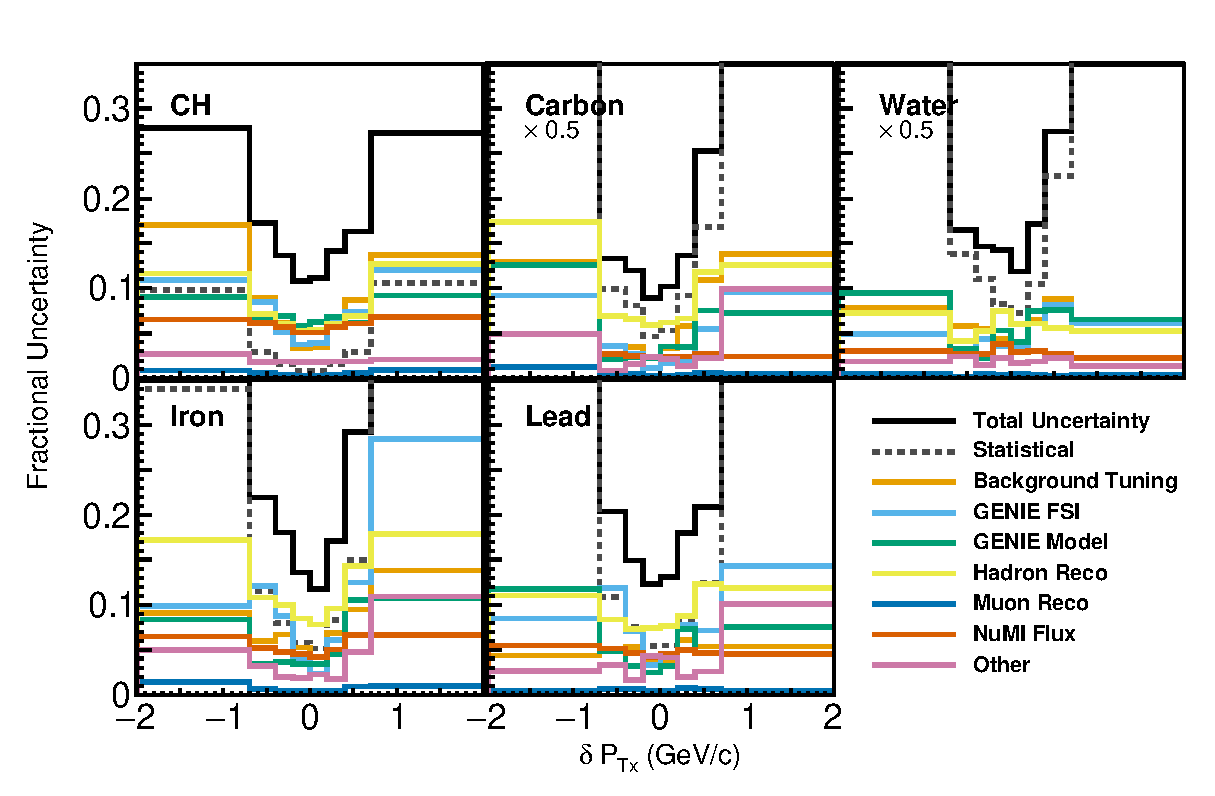
\includegraphics[width=\linewidth]{Figures/xsec_errors_all5/errors_dptx.eps}
    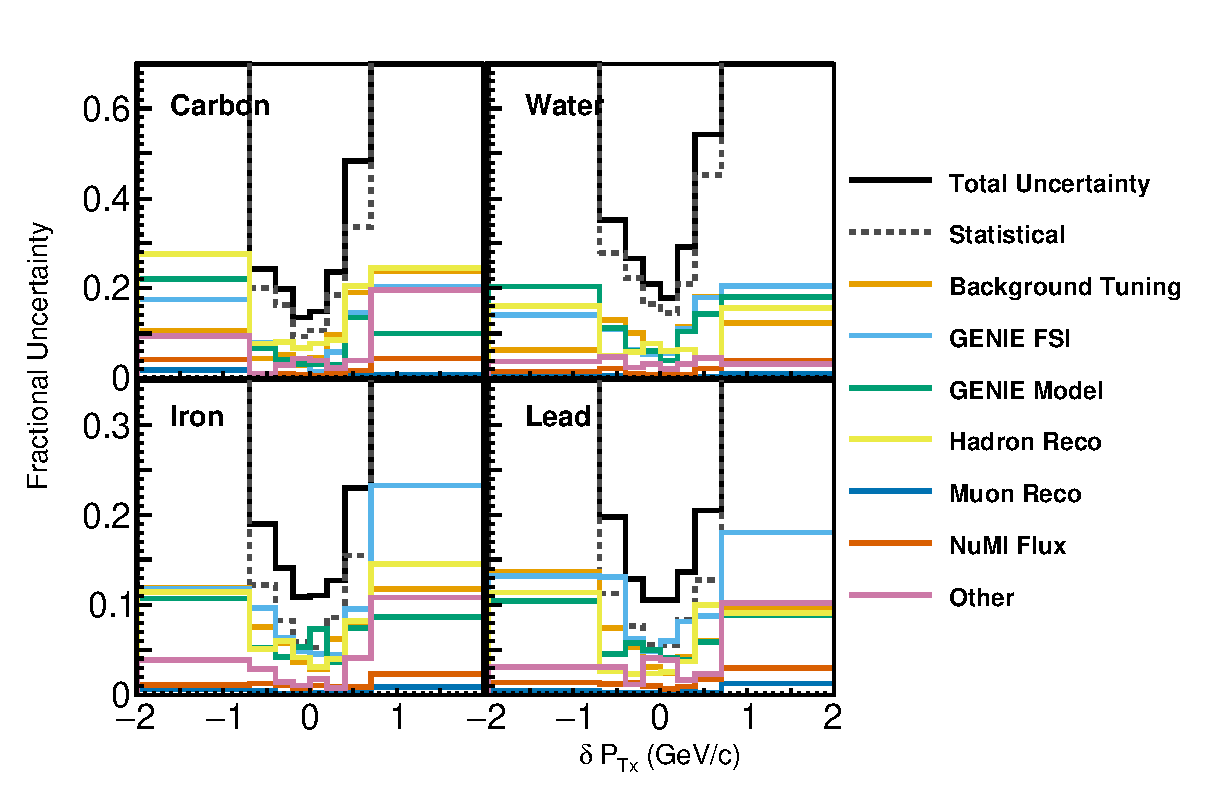
\includegraphics[width=\linewidth]{Figures/xsec_ratio_errors/ratio_errors_dptx.eps}
    \caption[\tkidptx cross-section uncertainties for multiple targets]{Uncertainties on the absolute cross section for each target (upper five plots) and on the ratio to CH (lower four plots) as a function of \tkidptx.}
    \label{fig:xsec_err_dptx}
\end{figure}
% dpty
\begin{figure}
	\centering
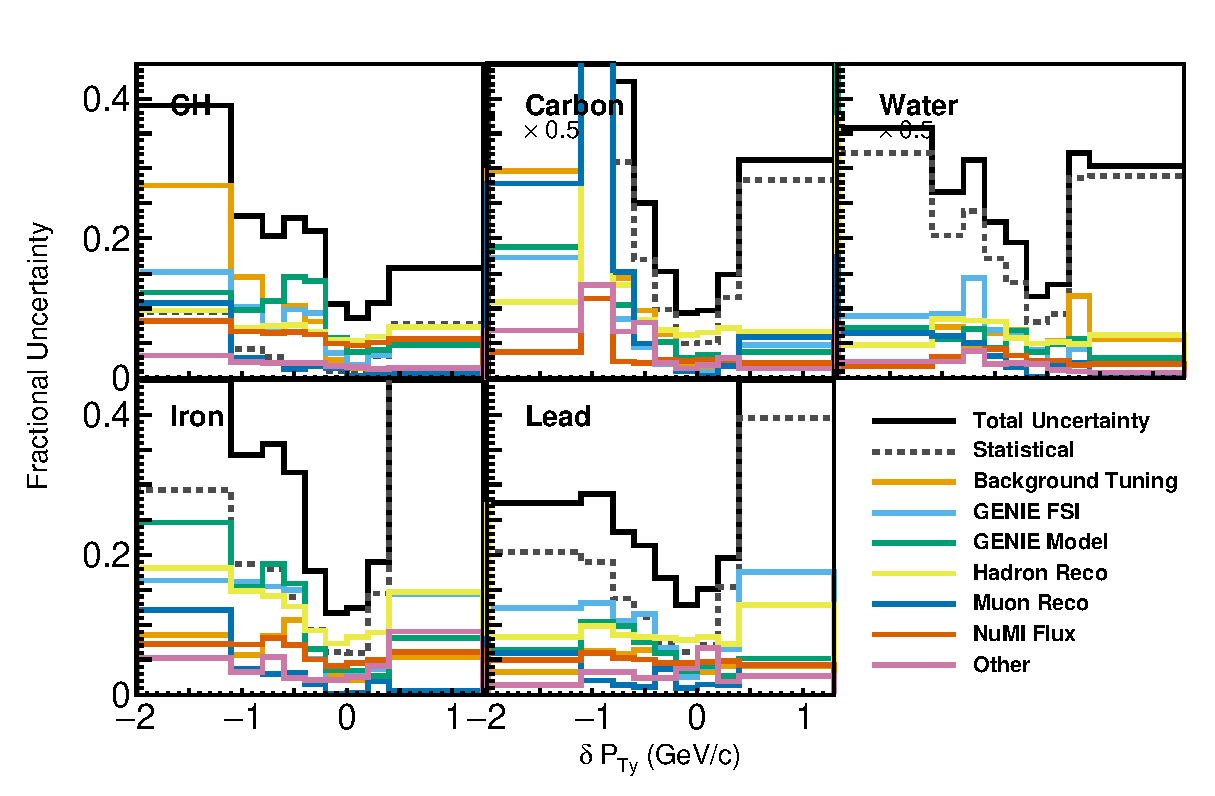
\includegraphics[width=\linewidth]{Figures/xsec_errors_all5/errors_dpty.eps}
    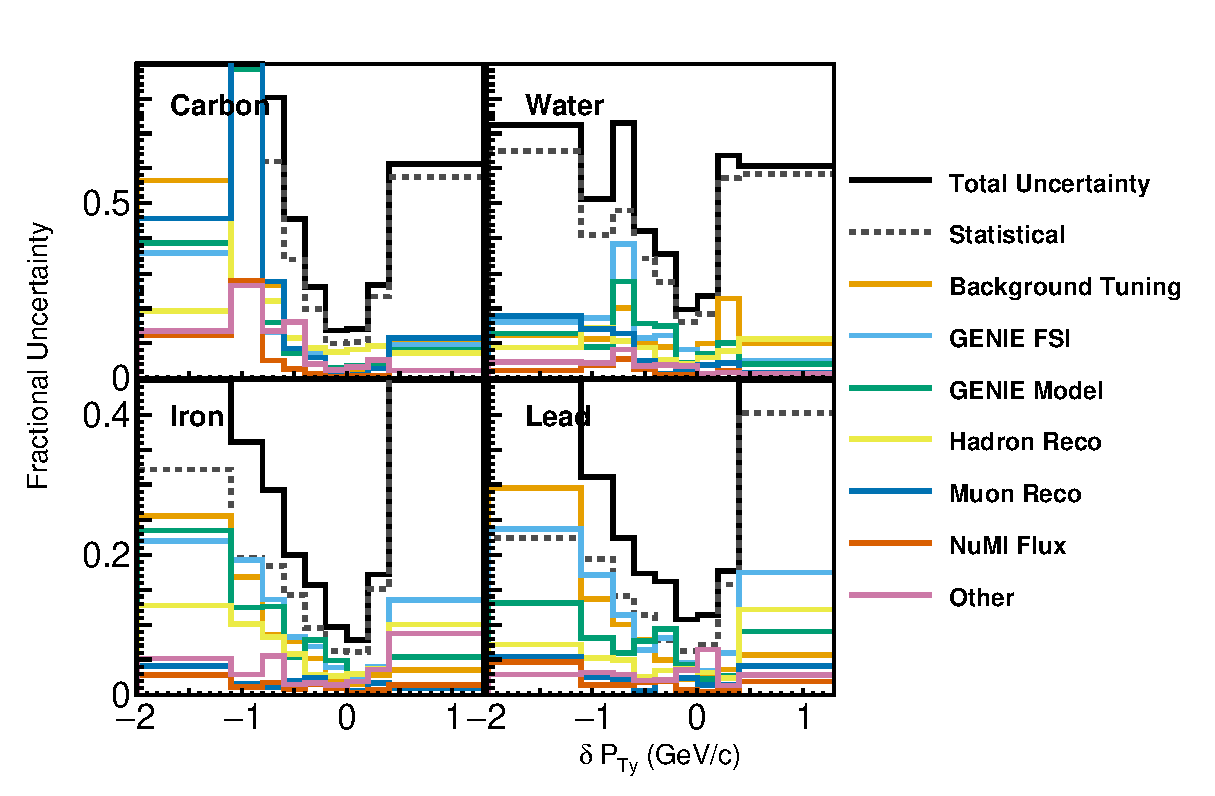
\includegraphics[width=\linewidth]{Figures/xsec_ratio_errors/ratio_errors_dpty.eps}
    \caption[\tkidpty cross-section uncertainties for multiple target ratios]{Uncertainties on the absolute cross section for each target (upper five plots) and on the ratio to CH (lower four plots) as a function of \tkidpty.}
    \label{fig:xsec_err_dpty}
\end{figure}
% dpl
\begin{figure}
	\centering
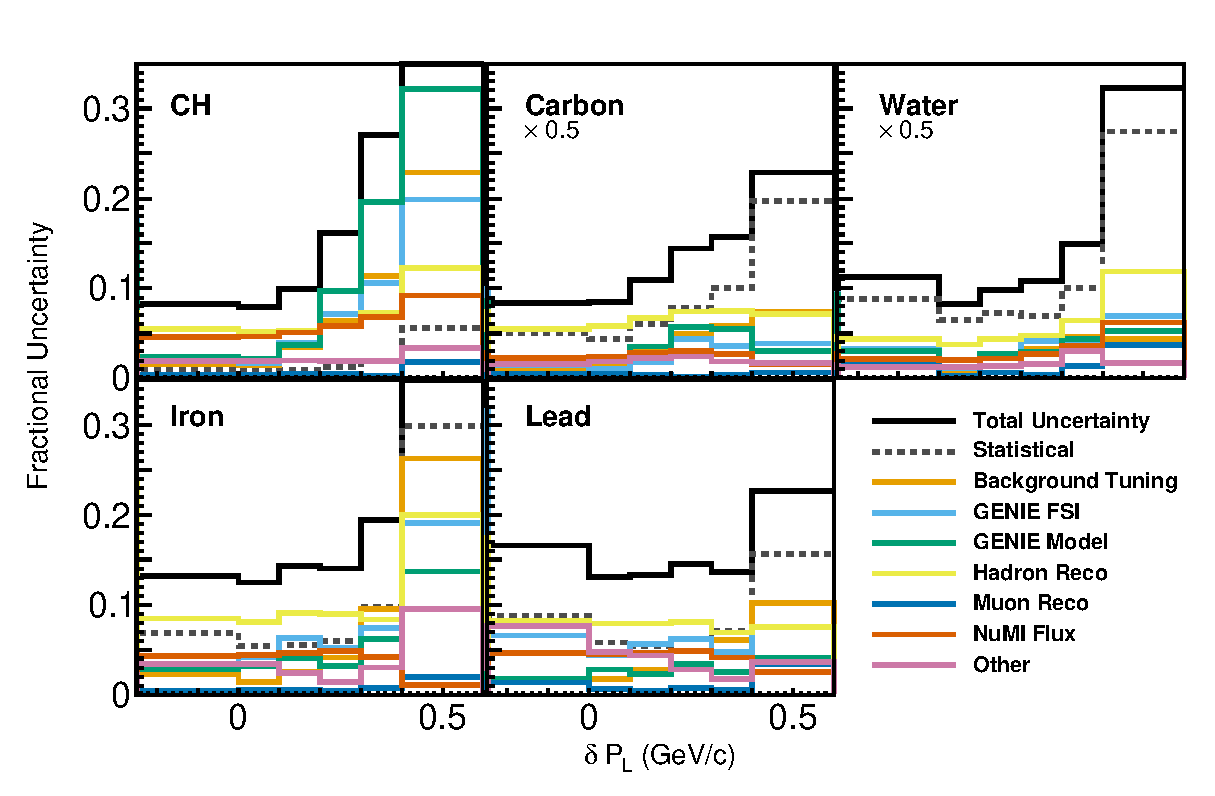
\includegraphics[width=\linewidth]{Figures/xsec_errors_all5/errors_pl.eps}
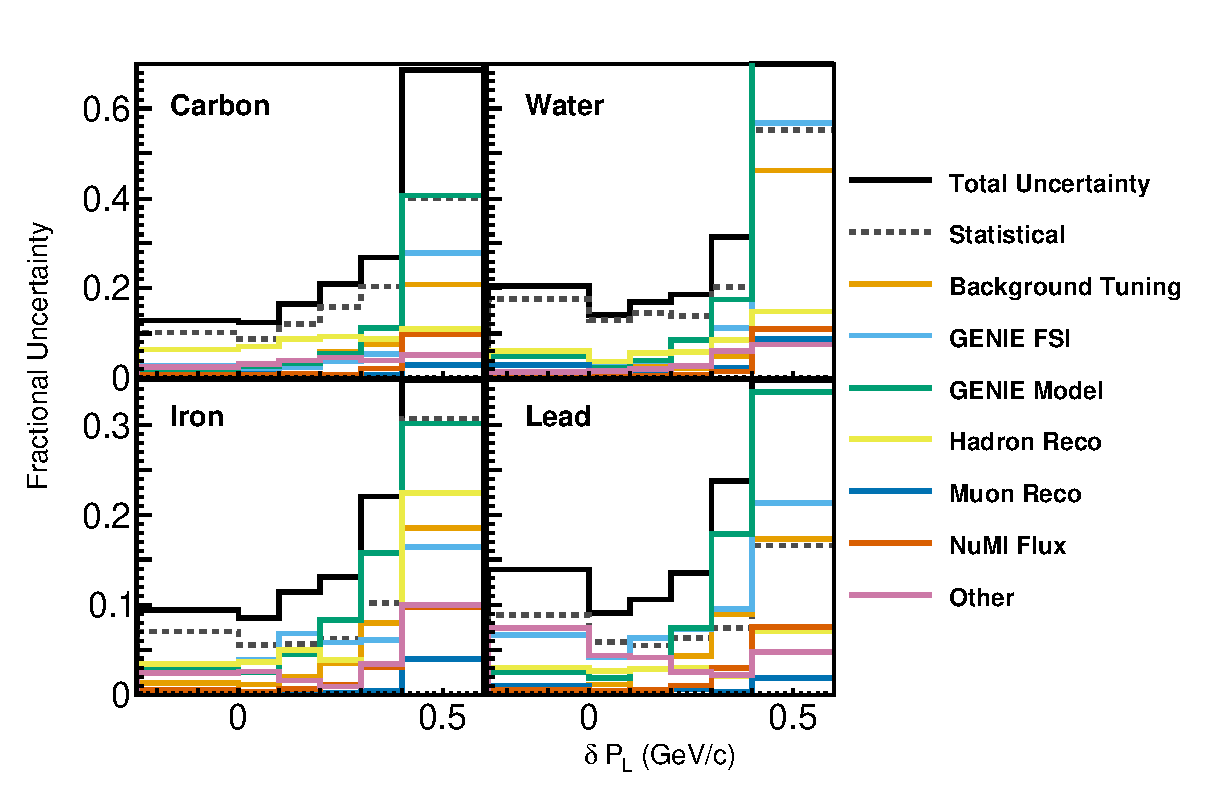
\includegraphics[width=\linewidth]{Figures/xsec_ratio_errors/ratio_errors_pl.eps}    \caption[\tkipl cross-section uncertainties for multiple targets]{Uncertainties on the absolute cross section for each target (upper five plots) and on the ratio to CH (lower four plots) as a function of \tkipl.}
    \label{fig:xsec_err_pl}
\end{figure}
% pn
\begin{figure}
	\centering
    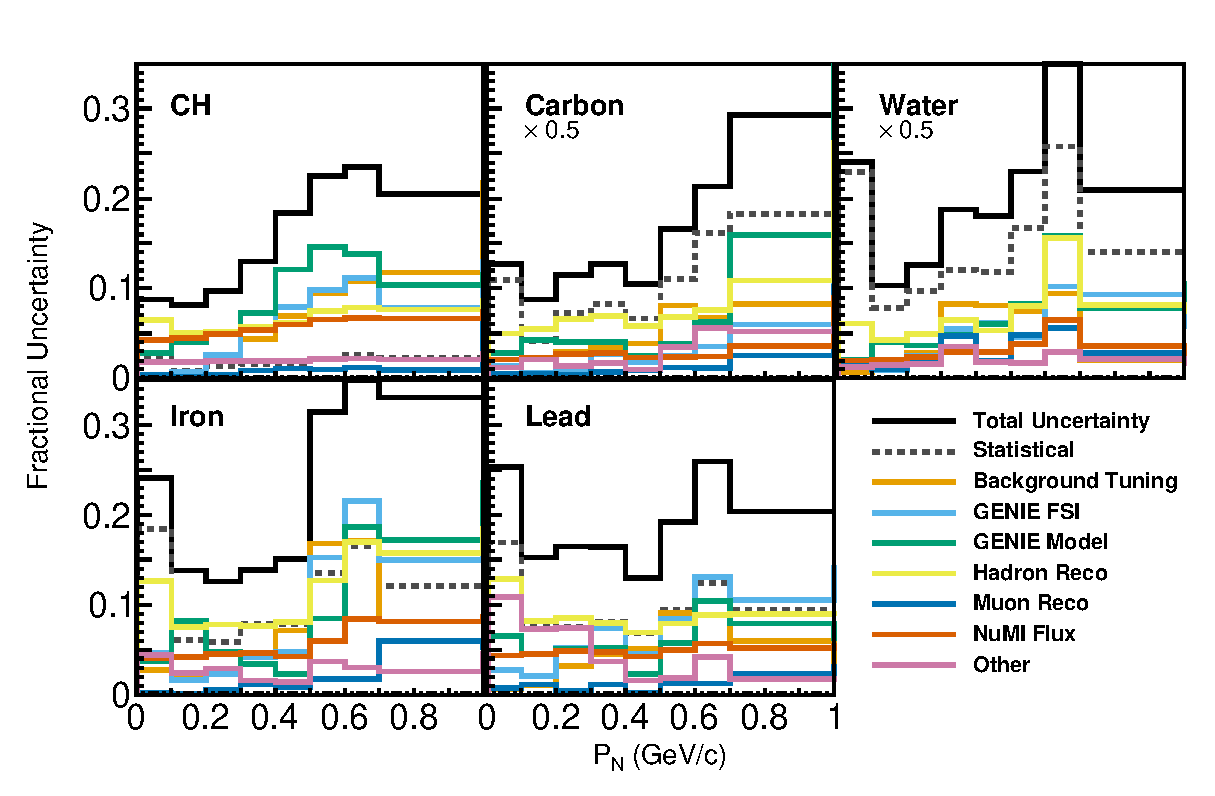
\includegraphics[width=\linewidth]{Figures/xsec_errors_all5/errors_pn.eps}
    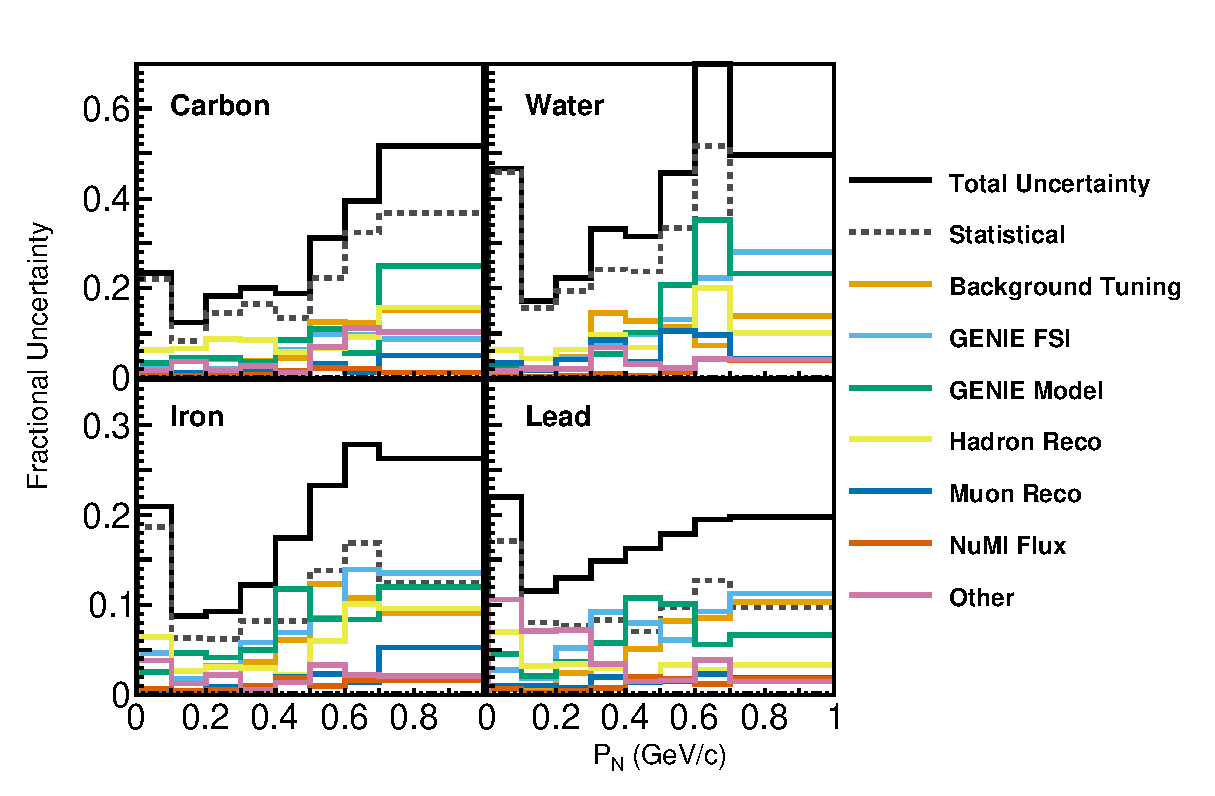
\includegraphics[width=\linewidth]{Figures/xsec_ratio_errors/ratio_errors_pn.eps}\caption[\tkipn cross-section ratio uncertainties for multiple targets]{Uncertainties on the absolute cross section for each target (upper five plots) and on the ratio to CH (lower four plots) as a function of \tkipn .}
    \label{fig:xsec_err_pn}
\end{figure}
% p_muon
\begin{figure}
	\centering
    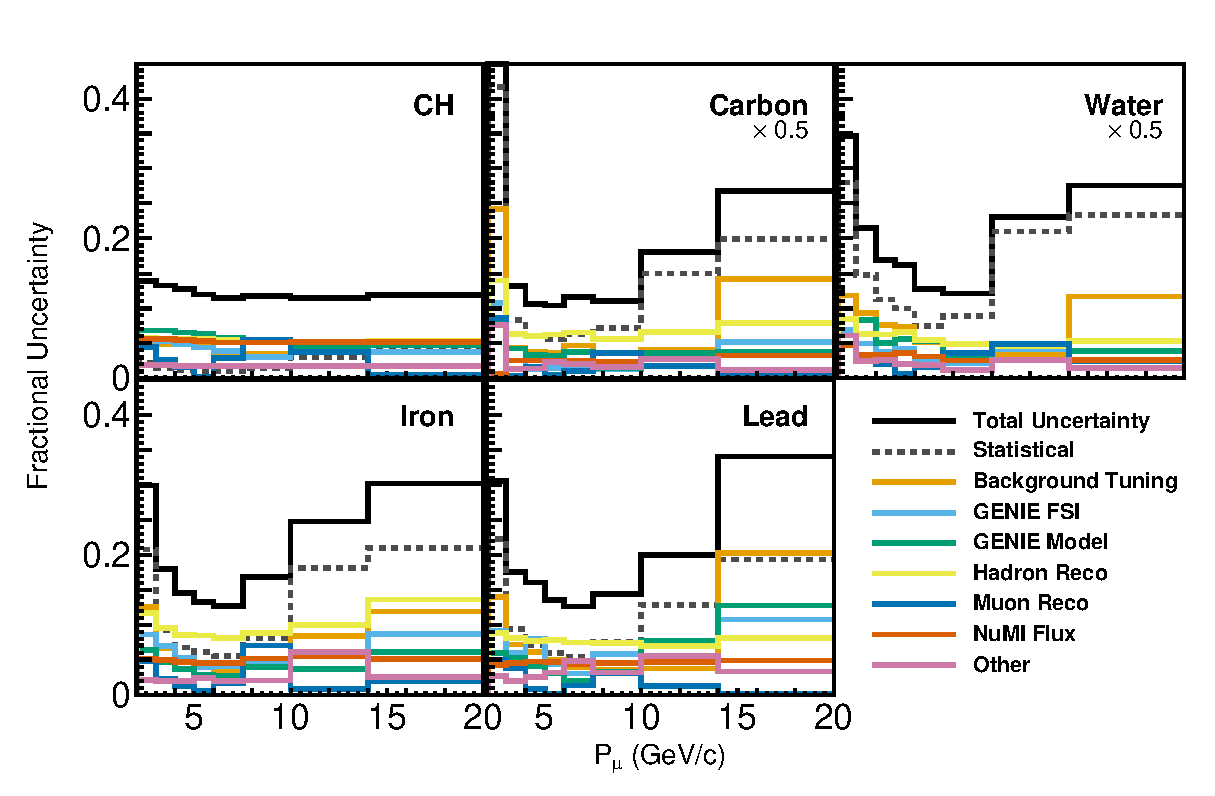
\includegraphics[width=\linewidth]{Figures/xsec_errors_all5/errors_muon_p.eps}
        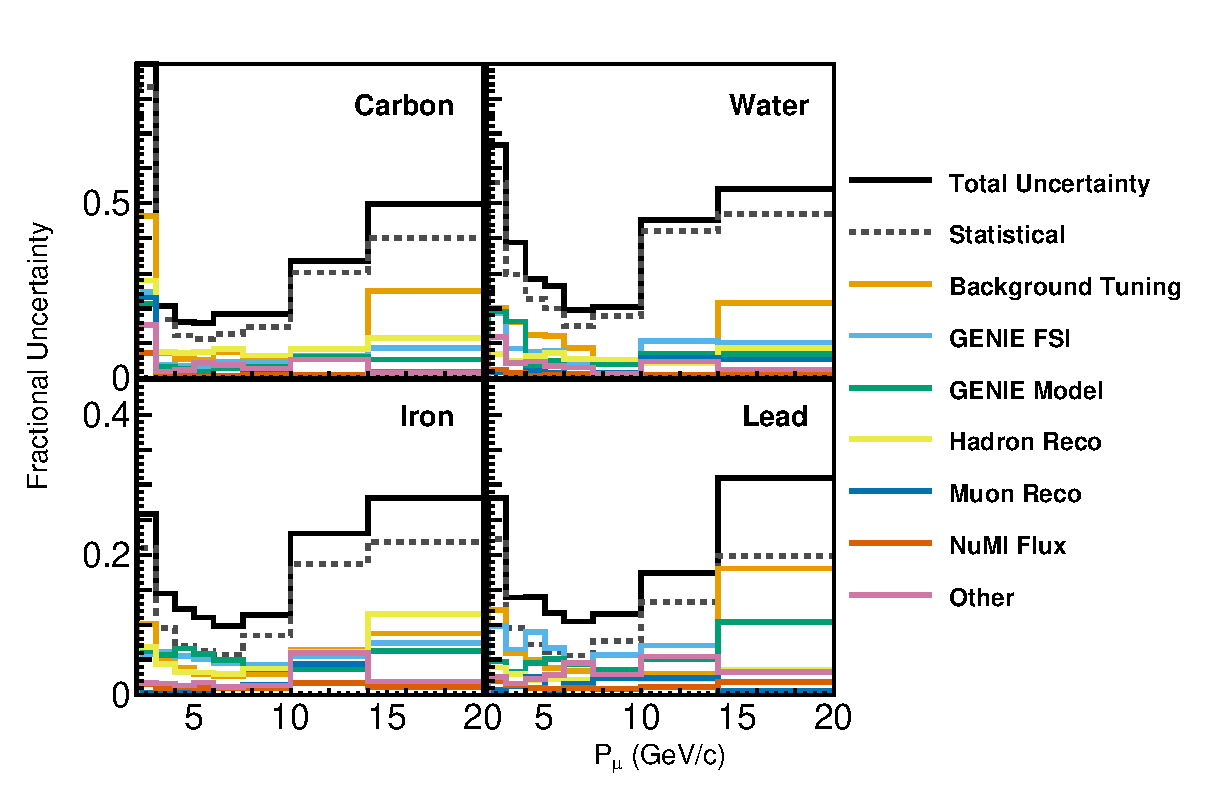
\includegraphics[width=\linewidth]{Figures/xsec_ratio_errors/ratio_errors_muon_p.eps}

    \caption[Muon momentum cross-section uncertainties for multiple targets ]{Uncertainties on the absolute cross section for each target (upper five plots) and on the ratio to CH (lower four plots) as a function of muon momentum.}
    \label{fig:xsec_err_muon_p}
\end{figure}
% pt_muon
\begin{figure}
	\centering
    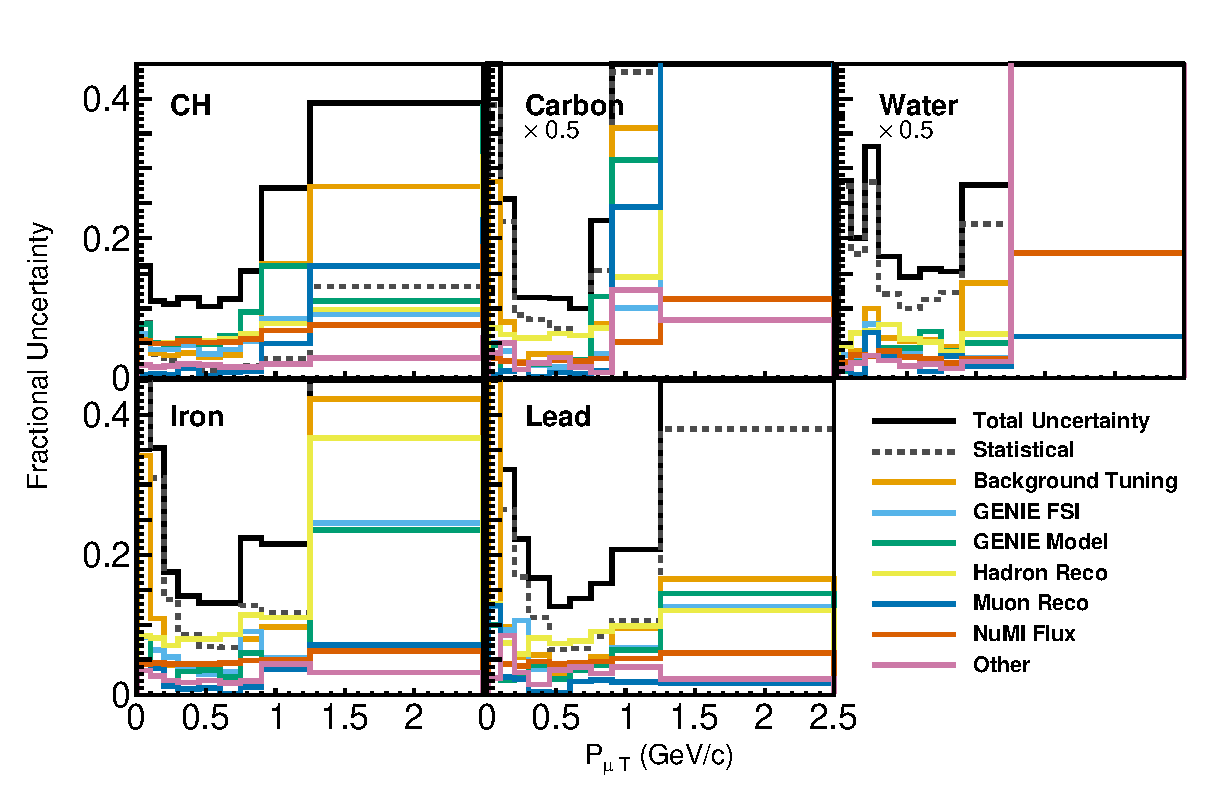
\includegraphics[width=\linewidth]{Figures/xsec_errors_all5/errors_muon_pt.eps}
        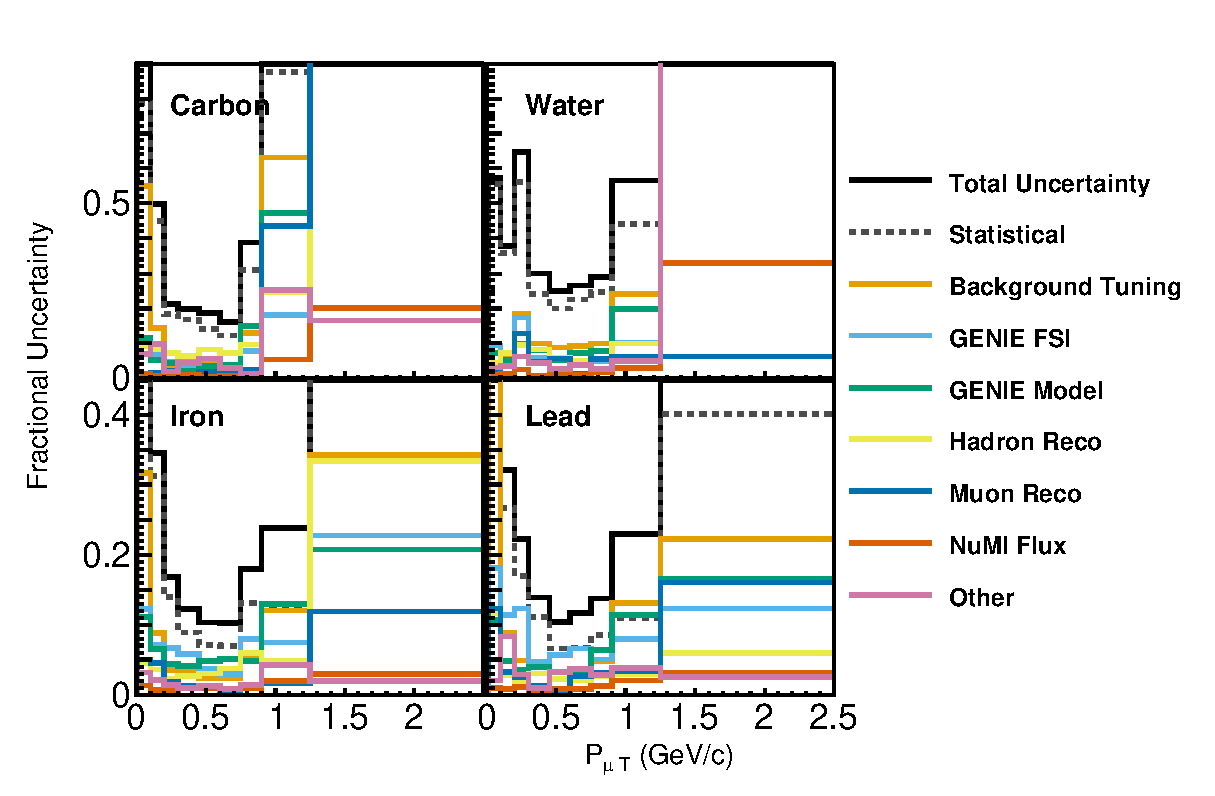
\includegraphics[width=\linewidth]{Figures/xsec_ratio_errors/ratio_errors_muon_pt.eps}
    \caption[Muon transverse momentum cross-section uncertainties for multiple targets]{Uncertainties on the absolute cross section for each target (upper five plots) and on the ratio to CH (lower four plots) as a function of muon transverse momentum.}
    \label{fig:xsec_err_muon_pt}
\end{figure}
% theta_muon
\begin{figure}
	\centering
    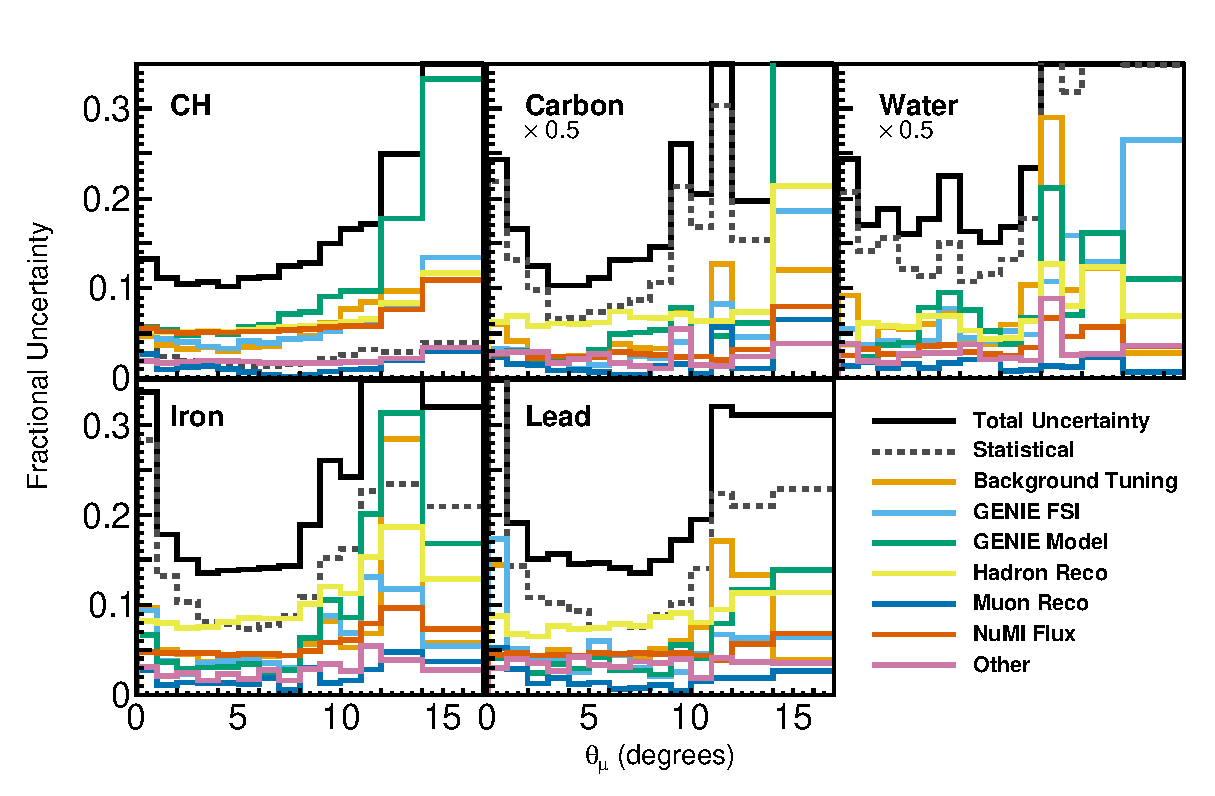
\includegraphics[width=\linewidth]{Figures/xsec_errors_all5/errors_muon_theta.eps}
    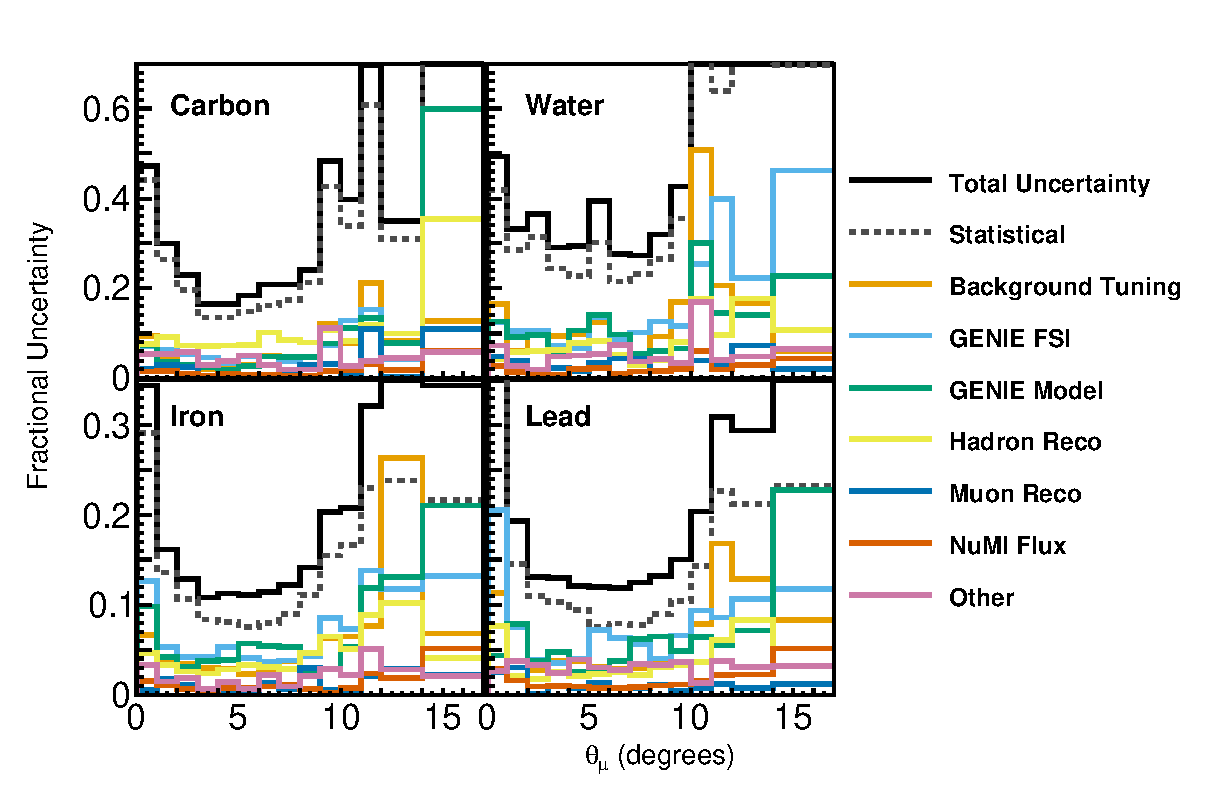
\includegraphics[width=\linewidth]{Figures/xsec_ratio_errors/ratio_errors_muon_theta.eps}
    \caption[$\theta_\mu$ cross-section uncertainties for multiple targets ]{Uncertainties on the absolute cross section for each target (upper five plots) and on the ratio to CH (lower four plots) as a function of $\theta_\mu$.}
    \label{fig:xsec_err_muon_theta}
\end{figure}
% p_proton
\begin{figure}
	\centering
    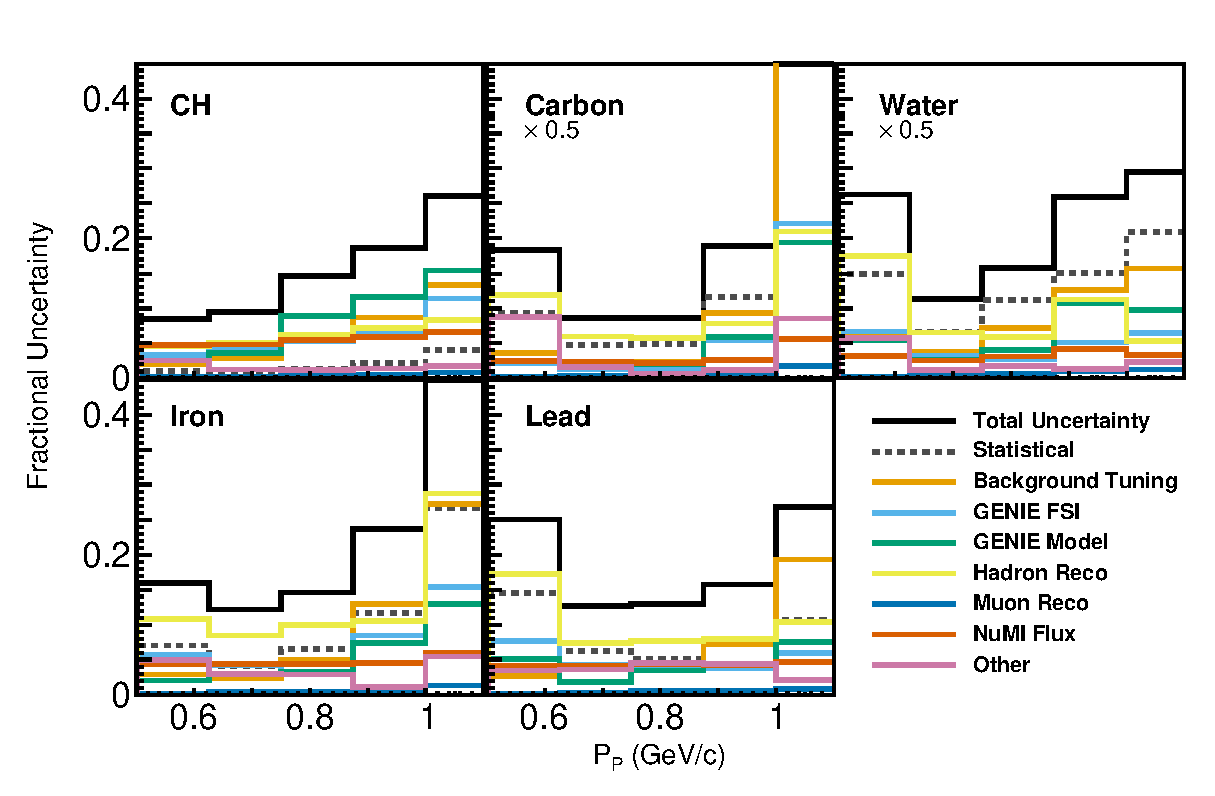
\includegraphics[width=\linewidth]{Figures/xsec_errors_all5/errors_proton_p.eps}
        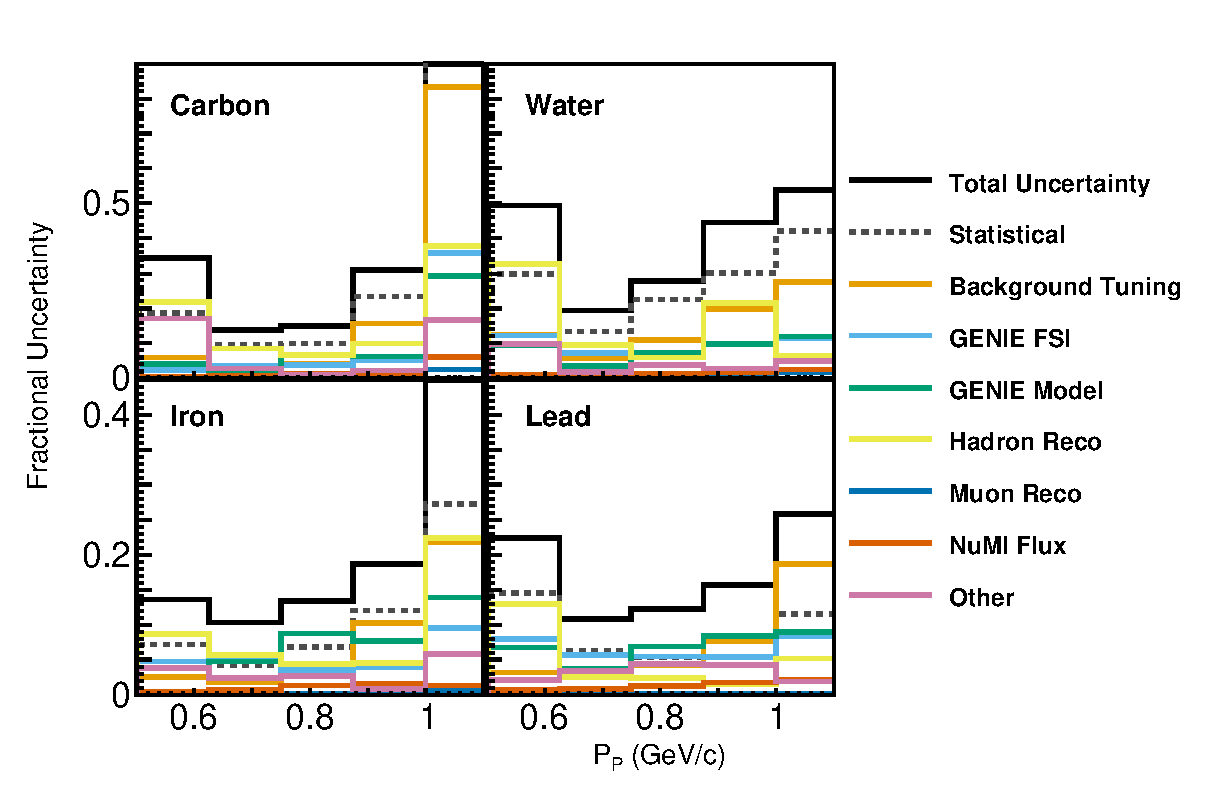
\includegraphics[width=\linewidth]{Figures/xsec_ratio_errors/ratio_errors_proton_p.eps}
    \caption[Proton momentum cross-section uncertainties for multiple targets ]{Uncertainties on the absolute cross section for each target (upper five plots) and on the ratio to CH (lower four plots) as a function of proton momentum.}
    \label{fig:xsec_err_proton_p}
\end{figure}
% pt_proton
\begin{figure}
	\centering
    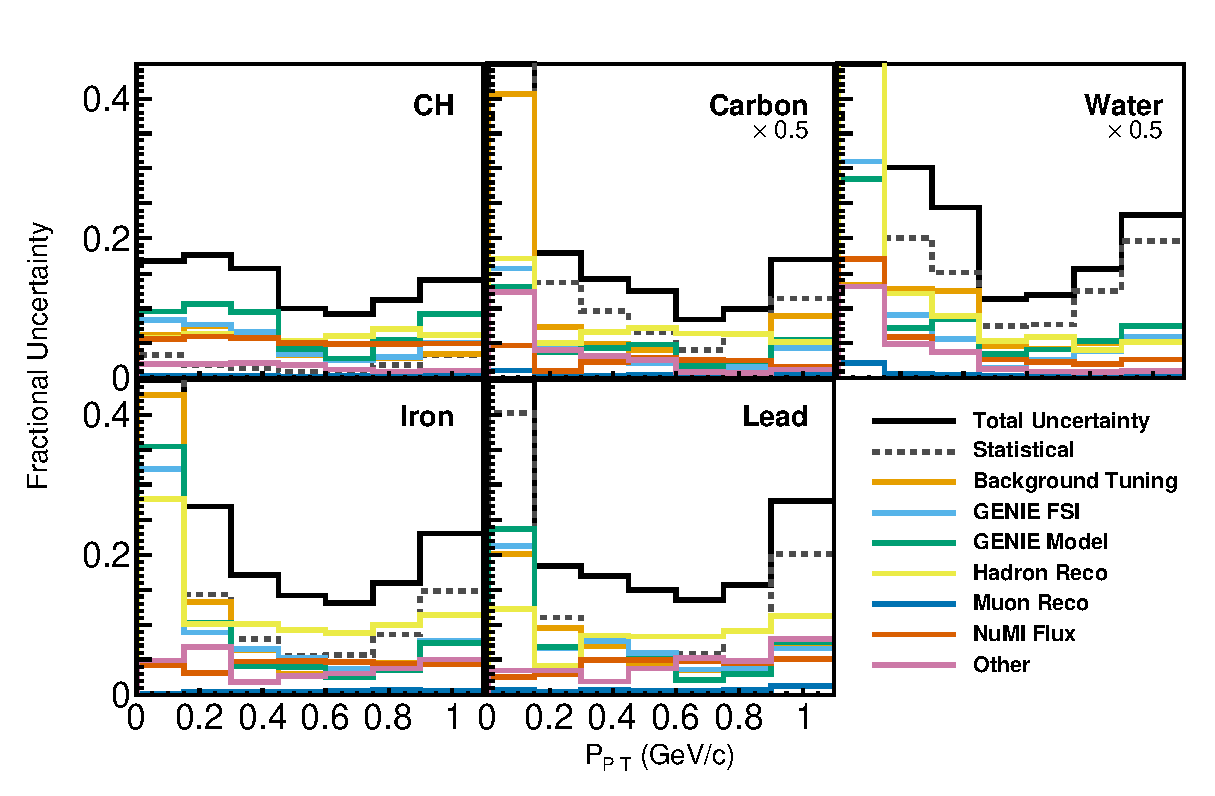
\includegraphics[width=\linewidth]{Figures/xsec_errors_all5/errors_proton_pt.eps}
        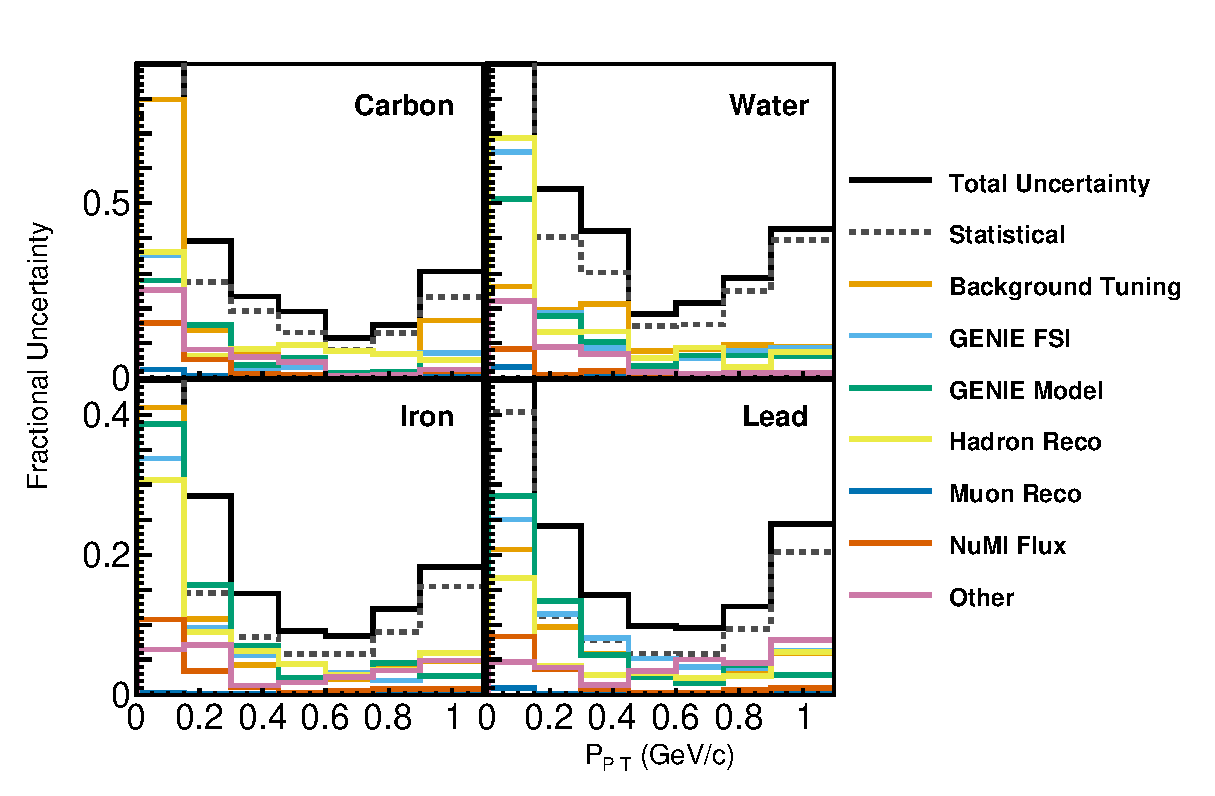
\includegraphics[width=\linewidth]{Figures/xsec_ratio_errors/ratio_errors_proton_pt.eps}
    \caption[cross-section uncertainties for multiple targets ]{Uncertainties on the absolute cross section for each target (upper five plots) and on the ratio to CH (lower four plots) as a function of proton transverse momentum.}
    \label{fig:xsec_err_proton_pt}
\end{figure}
% theta_proton
\begin{figure}
	\centering
    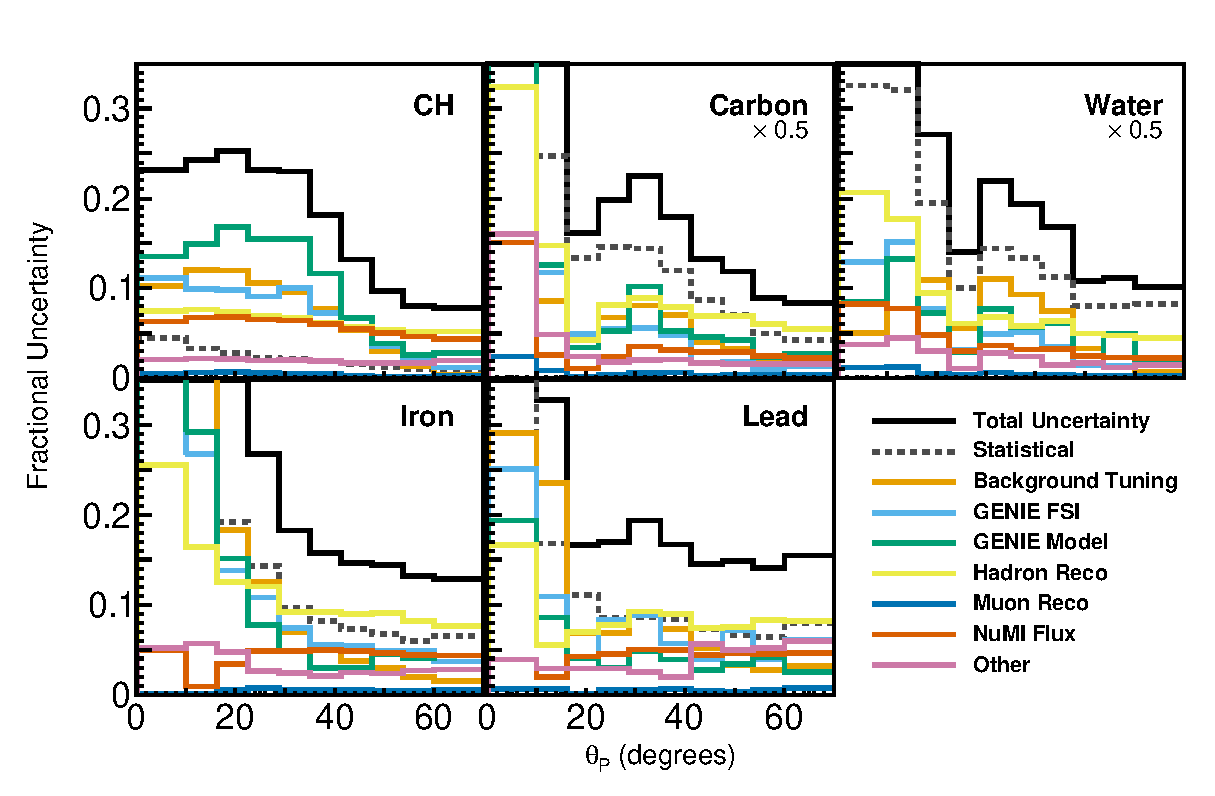
\includegraphics[width=\linewidth]{Figures/xsec_errors_all5/errors_proton_theta.eps}
    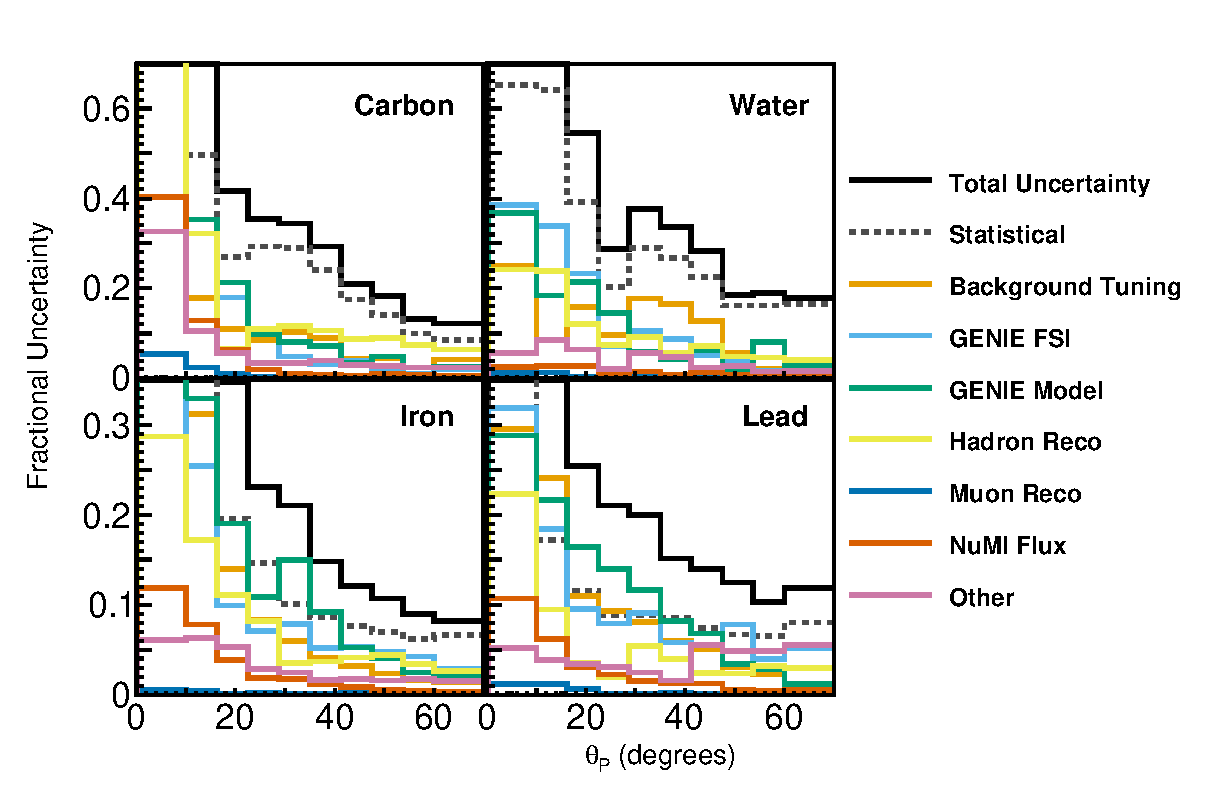
\includegraphics[width=\linewidth]{Figures/xsec_ratio_errors/ratio_errors_proton_theta.eps}
    \caption[$\theta_p$ cross-section uncertainties for multiple targets ]{Uncertainties on the absolute cross section for each target (upper five plots) and on the ratio to CH (lower four plots) as a function of proton angle with respect to the neutrino beam.}
    \label{fig:xsec_err_proton_theta}
\end{figure}

\clearpage
% dalphat chi2 table:
\section{Comparisons of \chisq\ between models and measurements }
\label{sect:chi2tables}
This section summarizes the comparisons between the measured cross sections and the different predictions described in Table~\ref{tab:generators} by listing the \chisq\ between the measured cross section and the prediction from each generator.  All correlations in the measurement uncertainties are taken into account:  both those between bins in one distribution and those between any passive target and the scintillator cross section.  The number of degrees of freedom, $N{dof}$ is provided in each table's caption.  

\begin{table*}[h]
    \centering
    \begin{tabular}{|Q|P|P|P|P|P|P|P|P|P|}
    \hline
    Model & CH \chisq & C & C/CH & \water & \water/CH & Fe & Fe/CH & Pb & Pb/CH \\ \hline
    Minerva Tune & 26 & 7.8 & 5.4 & 0.51 & 1.1 & 5.0 & 4.5 & 44 & 31  \\ \hline
    GENIEv3 G18 01a & 4.3 & 7.8 & 5.5 & 2.6 & 1.6 & 1.6 & 1.8 & 41 & 21  \\ \hline
    GENIEv3 G18 01b & 5.3 & 7.8 & 6.0 & 2.8 & 1.4 & 9.2 & 5.4 & 29 & 27  \\ \hline
    GENIEv3 G18 10a & 9.2 & 15 & 6.2 & 2.2 & 1.5 & 5.1 & 3.3 & 45 & 35  \\ \hline
    GENIEv3 G18 10b & 8.5 & 12 & 6.3 & 3.1 & 1.7 & 23 & 10 & 53 & 44  \\ \hline
    GiBUU T0 & 6.3 & 5.2 & 5.2 & 0.66 & 0.92 & 7.4 & 8.9 & 6.7 & 13  \\ \hline
    GiBUU T1 & 19 & 5.2 & 6.1 & 0.66 & 1.7 & 7.4 & 3.3 & 6.7 & 10  \\ \hline
    NEUT LFG & 44 & 32 & 5.5 & 4.7 & 0.77 & 60 & 4.1 & 140 & 21  \\ \hline
    NuWro LFG & 71 & 18 & 5.0 & 10 & 1.8 & 9.9 & 4.9 & 49 & 6.7  \\ \hline
    NuWro SF & 5.1 & 6.8 & 5.4 & 3.4 & 2.0 & 17 & 12 & 160 & 88  \\ \hline
    \end{tabular}
    \caption{Comparison of models and data for \tkialpha cross sections  corresponding to Figs. 
    \ref{fig:models_alphat} and \ref{Figure:Gencompare_alpha_ratio}, with $\ndf=5$.}
    \label{tab:dalphat}
\end{table*}
% dalphat chi2 table end


% dpt chi2 table:
\begin{table*}[h]
    \centering
    \begin{tabular}{|Q|P|P|P|P|P|P|P|P|P|}
    \hline
    Model & CH \chisq & C & C/CH & \water & \water/CH & Fe & Fe/CH & Pb & Pb/CH \\ \hline
    Minerva Tune & 35 & 5.9 & 3.6 & 8.3 & 3.0 & 13 & 8.5 & 35 & 21  \\ \hline
    GENIEv3 G18 01a & 29 & 4.5 & 3.2 & 6.9 & 1.2 & 16 & 7.5 & 21 & 13  \\ \hline
    GENIEv3 G18 01b & 32 & 5.4 & 5.2 & 10 & 1.5 & 30 & 8.9 & 84 & 27  \\ \hline
    GENIEv3 G18 10a & 140 & 24 & 5.1 & 8.4 & 0.88 & 17 & 10 & 39 & 26  \\ \hline
    GENIEv3 G18 10b & 130 & 20 & 5.2 & 11 & 1.4 & 28 & 19 & 100 & 62  \\ \hline
    GiBUU T0 & 21 & 2.2 & 3.0 & 5.1 & 1.8 & 20 & 7.7 & 27 & 21  \\ \hline
    GiBUU T1 & 41 & 2.2 & 5.2 & 5.1 & 1.7 & 20 & 6.1 & 27 & 14  \\ \hline
    NEUT LFG & 120 & 18 & 2.1 & 20 & 3.4 & 49 & 4.8 & 210 & 20  \\ \hline
    NuWro LFG & 250 & 32 & 3.8 & 5.3 & 0.72 & 25 & 7.6 & 42 & 11  \\ \hline
    NuWro SF & 55 & 8.3 & 4.0 & 3.9 & 0.7 & 32 & 39 & 140 & 110  \\ \hline
    \end{tabular}
    \caption{Comparison of models and data for \tkidelta cross sections  corresponding to Figs. \ref{Figure:Gencompare_dpt} and \ref{Figure:Gencompare_dpt_ratio}, with $\ndf=6$.}
    \label{tab:dpt}
\end{table*}
% dpt chi2 table end

% dptx chi2 table:
\begin{table*}[h]
    \centering
    \begin{tabular}{|Q|P|P|P|P|P|P|P|P|P|}
    \hline
    Model & CH \chisq & C & C/CH & \water & \water/CH & Fe & Fe/CH & Pb & Pb/CH \\ \hline
    Minerva Tune & 85 & 6.2 & 5.4 & 6.8 & 4.9 & 8.8 & 11 & 6.2 & 19  \\ \hline
    GENIEv3 G18 01a & 170 & 4.8 & 5.1 & 7.5 & 3.5 & 13 & 9.5 & 5.0 & 9.0  \\ \hline
    GENIEv3 G18 01b & 250 & 7.7 & 6.4 & 11 & 3.3 & 20 & 21 & 61 & 50  \\ \hline
    GENIEv3 G18 10a & 110 & 10 & 6.9 & 6.5 & 3.8 & 20 & 14 & 15 & 12  \\ \hline
    GENIEv3 G18 10b & 220 & 11 & 7.8 & 9.5 & 4.0 & 31 & 28 & 84 & 82  \\ \hline
    GiBUU T0 & 23 & 3.3 & 4.9 & 4.7 & 3.9 & 9.8 & 15 & 6.3 & 12  \\ \hline
    GiBUU T1 & 48 & 3.3 & 6.3 & 4.7 & 4.8 & 9.8 & 13 & 6.3 & 7.5  \\ \hline
    NEUT LFG & 120 & 19 & 4.3 & 11 & 5.1 & 56 & 12 & 160 & 45  \\ \hline
    NuWro LFG & 240 & 13 & 5.6 & 5.8 & 3.9 & 18 & 10 & 12 & 9.6  \\ \hline
    NuWro SF & 100 & 5.5 & 5.9 & 5.4 & 3.6 & 19 & 20 & 26 & 34  \\ \hline
    \end{tabular}
    \caption{Comparison of models and data for \tkidptx cross sections  corresponding to Figs. \ref{fig:models_dptx} and \ref{Fig:ratios_dptx}, with $\ndf=8$.}
    \label{tab:dptx}
\end{table*}
% dptx chi2 table end

% dpty chi2 table:
\begin{table*}[h]
    \centering
    \begin{tabular}{|Q|P|P|P|P|P|P|P|P|P|}
    \hline
    Model & CH \chisq & C & C/CH & \water & \water/CH & Fe & Fe/CH & Pb & Pb/CH \\ \hline
    Minerva Tune & 140 & 28 & 11 & 4.7 & 5.2 & 8.7 & 4.7 & 32 & 22  \\ \hline
    GENIEv3 G18 01a & 56 & 19 & 11 & 8.9 & 5.3 & 11 & 4.3 & 44 & 17  \\ \hline
    GENIEv3 G18 01b & 45 & 21 & 13 & 9.9 & 5.1 & 20 & 7.2 & 51 & 34  \\ \hline
    GENIEv3 G18 10a & 92 & 47 & 14 & 3.2 & 5.1 & 10 & 4.6 & 37 & 26  \\ \hline
    GENIEv3 G18 10b & 72 & 44 & 14 & 5.2 & 5.3 & 21 & 13 & 55 & 53  \\ \hline
    GiBUU T0 & 18 & 9.9 & 10 & 6.3 & 5.0 & 10 & 8.6 & 16 & 18  \\ \hline
    GiBUU T1 & 28 & 9.9 & 9.5 & 6.3 & 5.2 & 10 & 4.3 & 16 & 12  \\ \hline
    NEUT LFG & 120 & 69 & 11 & 9.7 & 6.0 & 45 & 3.6 & 120 & 26  \\ \hline
    NuWro LFG & 160 & 33 & 11 & 7.7 & 5.2 & 9.2 & 5.3 & 39 & 7.4  \\ \hline
    NuWro SF & 150 & 24 & 11 & 7.9 & 5.5 & 20 & 13 & 120 & 70  \\ \hline
    \end{tabular}
    \caption{Comparison of models and data for \tkidpty cross sections  corresponding to Figs. \ref{fig:models_dpty} and \ref{fig:ratiomodels_dpty}, with $\ndf=12$.}
    \label{tab:dpty}
\end{table*}
% dpty chi2 table end

% muonmomentum chi2 table:
\begin{table*}[h]
    \centering
    \begin{tabular}{|Q|P|P|P|P|P|P|P|P|P|}
    \hline
    Model & CH \chisq & C & C/CH & \water & \water/CH & Fe & Fe/CH & Pb & Pb/CH \\ \hline
    Minerva Tune & 57 & 23 & 12 & 4.4 & 4.9 & 4.0 & 5.0 & 9.7 & 16  \\ \hline
    GENIEv3 G18 01a & 350 & 30 & 14 & 5.0 & 5.1 & 13 & 2.8 & 21 & 9.6  \\ \hline
    GENIEv3 G18 01b & 310 & 37 & 17 & 5.0 & 5.3 & 16 & 4.5 & 72 & 33  \\ \hline
    GENIEv3 G18 10a & 400 & 41 & 16 & 5.6 & 5.5 & 15 & 2.4 & 28 & 8.3  \\ \hline
    GENIEv3 G18 10b & 410 & 43 & 17 & 5.7 & 5.3 & 27 & 8.8 & 110 & 43  \\ \hline
    GiBUU T0 & 33 & 16 & 12 & 4.5 & 4.8 & 3.3 & 6.1 & 21 & 21  \\ \hline
    GiBUU T1 & 38 & 16 & 12 & 4.5 & 5.4 & 3.3 & 2.9 & 21 & 15  \\ \hline
    NEUT LFG & 740 & 57 & 12 & 6.9 & 6.2 & 44 & 3.9 & 190 & 32  \\ \hline
    NuWro LFG & 370 & 39 & 15 & 4.7 & 5.7 & 12 & 4.4 & 28 & 11  \\ \hline
    NuWro SF & 280 & 32 & 16 & 4.9 & 5.6 & 12 & 4.0 & 20 & 8.2  \\ \hline
    \end{tabular}
    \caption{Comparison of models and data for P$_\mu$ cross sections  corresponding to Figs. \ref{fig:models_muon_p} and \ref{Figure:Gencompare_pmu_ratio}, with $\ndf=8$.}
    \label{tab:muonmomentum}
\end{table*}
% muonmomentum chi2 table end


% muonpt chi2 table:
\begin{table*}[h]
    \centering
    \begin{tabular}{|Q|P|P|P|P|P|P|P|P|P|}
    \hline
    Model & CH \chisq & C & C/CH & \water & \water/CH & Fe & Fe/CH & Pb & Pb/CH \\ \hline
    Minerva Tune & 200 & 12 & 11 & 5.0 & 4.8 & 54 & 21 & 45 & 16  \\ \hline
    GENIEv3 G18 01a & 360 & 9.4 & 10 & 12 & 4.1 & 39 & 23 & 64 & 18  \\ \hline
    GENIEv3 G18 01b & 360 & 12 & 12 & 13 & 4.1 & 79 & 38 & 190 & 70  \\ \hline
    GENIEv3 G18 10a & 110 & 16 & 12 & 7.2 & 4.2 & 53 & 21 & 51 & 18  \\ \hline
    GENIEv3 G18 10b & 120 & 16 & 12 & 5.7 & 4.4 & 100 & 38 & 150 & 64  \\ \hline
    GiBUU T0 & 92 & 11 & 9.9 & 3.1 & 4.6 & 50 & 35 & 46 & 38  \\ \hline
    GiBUU T1 & 86 & 11 & 8.9 & 3.1 & 5.4 & 50 & 32 & 46 & 34  \\ \hline
    NEUT LFG & 140 & 23 & 8.4 & 10 & 5.5 & 140 & 30 & 330 & 82  \\ \hline
    NuWro LFG & 130 & 14 & 10 & 4.9 & 3.9 & 67 & 23 & 79 & 18  \\ \hline
    NuWro SF & 160 & 11 & 10 & 7.0 & 4.3 & 79 & 23 & 110 & 22  \\ \hline
    \end{tabular}
    \caption{Comparison of models and data for \tkiptmu cross sections  corresponding to Figs. \ref{Figure:Gencompare_ptmu} and \ref{Figure:Gencompare_ptmu_ratio}, with $\ndf=10$.}
    \label{tab:muonpt}
\end{table*}
% muonpt chi2 table end


% muontheta chi2 table:
\begin{table*}[h]
    \centering
    \begin{tabular}{|Q|P|P|P|P|P|P|P|P|P|}
    \hline
    Model & CH \chisq & C & C/CH & \water & \water/CH & Fe & Fe/CH & Pb & Pb/CH \\ \hline
    Minerva Tune & 130 & 16 & 15 & 8.0 & 6.1 & 21 & 10 & 64 & 28  \\ \hline
    GENIEv3 G18 01a & 170 & 10 & 15 & 10 & 6.3 & 28 & 9.8 & 91 & 35  \\ \hline
    GENIEv3 G18 01b & 240 & 14 & 17 & 13 & 6.6 & 63 & 17 & 260 & 90  \\ \hline
    GENIEv3 G18 10a & 250 & 20 & 17 & 7.2 & 6.1 & 38 & 9.6 & 110 & 39  \\ \hline
    GENIEv3 G18 10b & 360 & 25 & 17 & 9.9 & 7.2 & 82 & 23 & 250 & 87  \\ \hline
    GiBUU T0 & 54 & 13 & 14 & 6.6 & 5.9 & 18 & 16 & 55 & 50  \\ \hline
    GiBUU T1 & 69 & 13 & 14 & 6.6 & 6.2 & 18 & 13 & 55 & 41  \\ \hline
    NEUT LFG & 280 & 29 & 13 & 11 & 6.6 & 100 & 14 & 380 & 89  \\ \hline
    NuWro LFG & 370 & 24 & 15 & 9.9 & 6.3 & 49 & 8.7 & 140 & 28  \\ \hline
    NuWro SF & 440 & 20 & 14 & 9.9 & 6.4 & 54 & 8.8 & 190 & 44  \\ \hline
    \end{tabular}
    \caption{Comparison of models and data for $\theta_{\mu}$ cross sections  corresponding to Figs. \ref{fig:models_muon_theta} and \ref{Figure:Gencompare_mutheta_ratio}, with $\ndf=14$.}
    \label{tab:muontheta}
\end{table*}
% muontheta chi2 table end


% neutronmomentum chi2 table:
\begin{table*}[h]
    \centering
    \begin{tabular}{|Q|P|P|P|P|P|P|P|P|P|}
    \hline
    Model & CH \chisq & C & C/CH & \water & \water/CH & Fe & Fe/CH & Pb & Pb/CH \\ \hline
    Minerva Tune & 120 & 16 & 12 & 4.7 & 6.6 & 17 & 11 & 98 & 53  \\ \hline
    GENIEv3 G18 01a & 140 & 18 & 11 & 5.3 & 5.2 & 27 & 10 & 91 & 46  \\ \hline
    GENIEv3 G18 01b & 140 & 21 & 15 & 7.3 & 5.5 & 39 & 16 & 93 & 61  \\ \hline
    GENIEv3 G18 10a & 420 & 52 & 14 & 21 & 6.3 & 49 & 17 & 59 & 68  \\ \hline
    GENIEv3 G18 10b & 440 & 51 & 14 & 24 & 6.8 & 60 & 30 & 79 & 110  \\ \hline
    GiBUU T0 & 200 & 28 & 11 & 7.3 & 6.5 & 25 & 37 & 29 & 42  \\ \hline
    GiBUU T1 & 240 & 28 & 11 & 7.3 & 6.8 & 25 & 34 & 29 & 32  \\ \hline
    NEUT LFG & 540 & 48 & 9.7 & 24 & 7.9 & 100 & 30 & 170 & 54  \\ \hline
    NuWro LFG & 780 & 70 & 12 & 38 & 6.2 & 64 & 18 & 50 & 35  \\ \hline
    NuWro SF & 70 & 19 & 11 & 9.3 & 6.5 & 83 & 78 & 170 & 170  \\ \hline
    \end{tabular}
    \caption{Comparison of models and data for \tkipn cross sections  corresponding to Figs. \ref{fig:models_pn} and \ref{Figure:Gencompare_pn_ratio}, with $\ndf=10$.}
    \label{tab:neutronmomentum}
\end{table*}
% neutronmomentum chi2 table end


% phi chi2 table:
\begin{table*}[h]
    \centering
    \begin{tabular}{|Q|P|P|P|P|P|P|P|P|P|}
    \hline
    Model & CH \chisq & C & C/CH & \water & \water/CH & Fe & Fe/CH & Pb & Pb/CH \\ \hline
    Minerva Tune & 100 & 13 & 7.9 & 1.5 & 2.0 & 5.4 & 5.4 & 23 & 21  \\ \hline
    GENIEv3 G18 01a & 120 & 9.4 & 7.3 & 1.2 & 1.3 & 9.3 & 3.1 & 9.6 & 17  \\ \hline
    GENIEv3 G18 01b & 120 & 12 & 9.5 & 2.6 & 1.5 & 23 & 5.7 & 52 & 36  \\ \hline
    GENIEv3 G18 10a & 210 & 30 & 9.6 & 5.2 & 1.6 & 18 & 4.4 & 13 & 34  \\ \hline
    GENIEv3 G18 10b & 240 & 33 & 11 & 6.5 & 1.7 & 30 & 17 & 78 & 100  \\ \hline
    GiBUU T0 & 14 & 7.0 & 6.7 & 1.6 & 1.6 & 7.0 & 5.0 & 2.5 & 11  \\ \hline
    GiBUU T1 & 17 & 7.0 & 9.3 & 1.6 & 2.1 & 7.0 & 1.5 & 2.5 & 6.0  \\ \hline
    NEUT LFG & 200 & 27 & 6.1 & 7.7 & 2.2 & 53 & 2.2 & 190 & 21  \\ \hline
    NuWro LFG & 250 & 42 & 8.3 & 8.6 & 1.7 & 14 & 5.3 & 12 & 22  \\ \hline
    NuWro SF & 110 & 16 & 8.0 & 2.2 & 1.7 & 22 & 19 & 63 & 49  \\ \hline
    \end{tabular}
    \caption{Comparison of models and data for \tkiphi cross sections  corresponding to Figs. \ref{fig:models_coplan} and \ref{Figure:Gencompare_phi_ratio}, with $\ndf=6$.}
    \label{tab:phi}
\end{table*}
% phi chi2 table end


% pl chi2 table:
\begin{table*}[h]
    \centering
    \begin{tabular}{|Q|P|P|P|P|P|P|P|P|P|}
    \hline
    Model & CH \chisq & C & C/CH & \water & \water/CH & Fe & Fe/CH & Pb & Pb/CH \\ \hline
    Minerva Tune & 57 & 14 & 7.4 & 6.0 & 8.1 & 5.6 & 5.6 & 11 & 9.7  \\ \hline
    GENIEv3 G18 01a & 630 & 460 & 8.3 & 97 & 6.2 & 230 & 2.5 & 210 & 11  \\ \hline
    GENIEv3 G18 01b & 250 & 190 & 10 & 36 & 5.5 & 170 & 4.1 & 890 & 96  \\ \hline
    GENIEv3 G18 10a & 1300 & 1100 & 9.5 & 240 & 5.9 & 580 & 3.1 & 490 & 18  \\ \hline
    GENIEv3 G18 10b & 360 & 400 & 12 & 82 & 4.2 & 300 & 10 & 1700 & 140  \\ \hline
    GiBUU T0 & 51 & 7.0 & 7.3 & 15 & 10 & 21 & 21 & 33 & 58  \\ \hline
    GiBUU T1 & 53 & 7.0 & 5.6 & 15 & 14 & 21 & 17 & 33 & 34  \\ \hline
    NEUT LFG & 520 & 390 & 9.1 & 110 & 9.8 & 550 & 4.2 & 3300 & 98  \\ \hline
    NuWro LFG & 190 & 92 & 8.0 & 11 & 9.1 & 49 & 8.4 & 180 & 21  \\ \hline
    NuWro SF & 140 & 81 & 7.0 & 10 & 9.9 & 17 & 13 & 28 & 23  \\ \hline
    \end{tabular}
    \caption{Comparison of models and data for \tkipl cross sections  corresponding to Figs. \ref{fig:models_pl} and \ref{Figure:Gencompare_pl_ratio}, with $\ndf=8$.}
    \label{tab:pl}
\end{table*}
% pl chi2 table end


% protonmomentum chi2 table:
\begin{table*}[h]
    \centering
    \begin{tabular}{|Q|P|P|P|P|P|P|P|P|P|}
    \hline
    Model & CH \chisq & C & C/CH & \water & \water/CH & Fe & Fe/CH & Pb & Pb/CH \\ \hline
    Minerva Tune & 4.0 & 13 & 8.4 & 0.62 & 0.81 & 11 & 17 & 11 & 11  \\ \hline
    GENIEv3 G18 01a & 6.6 & 8.5 & 7.7 & 1.8 & 0.59 & 4.0 & 11 & 26 & 14  \\ \hline
    GENIEv3 G18 01b & 33 & 13 & 9.3 & 4.2 & 0.92 & 11 & 7.3 & 210 & 130  \\ \hline
    GENIEv3 G18 10a & 4.2 & 17 & 9.7 & 1.9 & 0.72 & 8.7 & 7.1 & 37 & 25  \\ \hline
    GENIEv3 G18 10b & 28 & 19 & 10 & 4.4 & 1.1 & 25 & 8.0 & 290 & 190  \\ \hline
    GiBUU T0 & 6.2 & 9.6 & 8.2 & 0.54 & 0.62 & 13 & 12 & 40 & 71  \\ \hline
    GiBUU T1 & 2.3 & 9.6 & 8.9 & 0.54 & 0.99 & 13 & 15 & 40 & 47  \\ \hline
    NEUT LFG & 41 & 28 & 7.9 & 5.9 & 1.2 & 40 & 3.5 & 520 & 210  \\ \hline
    NuWro LFG & 8.0 & 16 & 8.6 & 1.3 & 0.55 & 11 & 10 & 44 & 32  \\ \hline
    NuWro SF & 1.5 & 11 & 8.6 & 0.43 & 0.52 & 19 & 24 & 14 & 13  \\ \hline
    \end{tabular}
    \caption{Comparison of models and data for P$_{p}$ cross sections  corresponding to Figs. \ref{fig:models_proton_p} and \ref{Figure:Gencompare_proton_p_ratio}, with $\ndf=5$.}
    \label{tab:protonmomentum}
\end{table*}
% protonmomentum chi2 table end


% protonpt chi2 table:
\begin{table*}[h]
    \centering
    \begin{tabular}{|Q|P|P|P|P|P|P|P|P|P|}
    \hline
    Model & CH \chisq & C & C/CH & \water & \water/CH & Fe & Fe/CH & Pb & Pb/CH \\ \hline
    Minerva Tune & 36 & 12 & 7.9 & 8.0 & 5.3 & 3.7 & 7.2 & 12 & 14  \\ \hline
    GENIEv3 G18 01a & 41 & 14 & 8.6 & 11 & 5.9 & 5.4 & 5.5 & 16 & 11  \\ \hline
    GENIEv3 G18 01b & 32 & 17 & 10 & 13 & 7.0 & 18 & 16 & 110 & 100  \\ \hline
    GENIEv3 G18 10a & 51 & 15 & 10 & 10 & 6.2 & 13 & 8.2 & 21 & 13  \\ \hline
    GENIEv3 G18 10b & 48 & 15 & 9.9 & 11 & 7.2 & 32 & 24 & 150 & 130  \\ \hline
    GiBUU T0 & 20 & 7.8 & 8.4 & 7.2 & 6.3 & 3.7 & 15 & 18 & 41  \\ \hline
    GiBUU T1 & 22 & 7.8 & 7.4 & 7.2 & 5.5 & 3.7 & 9.5 & 18 & 25  \\ \hline
    NEUT LFG & 140 & 41 & 11 & 31 & 8.5 & 66 & 11 & 310 & 95  \\ \hline
    NuWro LFG & 52 & 8.8 & 8.2 & 3.9 & 5.0 & 7.3 & 6.4 & 18 & 15  \\ \hline
    NuWro SF & 35 & 9.7 & 7.8 & 6.2 & 5.0 & 13 & 15 & 24 & 24  \\ \hline
    \end{tabular}
    \caption{Comparison of models and data for \tkiptproton cross sections  corresponding to Figs. \ref{fig:models_proton_pt} and \ref{Figure:Gencompare_proton_pt_ratio}, with $\ndf=7$.}
    \label{tab:protonpt}
\end{table*}
% protonpt chi2 table end


% protontheta chi2 table:
\begin{table*}[h]
    \centering
    \begin{tabular}{|Q|P|P|P|P|P|P|P|P|P|}
    \hline
    Model & CH \chisq & C & C/CH & \water & \water/CH & Fe & Fe/CH & Pb & Pb/CH \\ \hline
    Minerva Tune & 49 & 15 & 6.0 & 8.6 & 7.9 & 6.5 & 6.5 & 22 & 10  \\ \hline
    GENIEv3 G18 01a & 34 & 12 & 6.4 & 9.9 & 6.2 & 7.4 & 3.0 & 24 & 11  \\ \hline
    GENIEv3 G18 01b & 20 & 13 & 7.7 & 11 & 6.2 & 14 & 9.1 & 92 & 93  \\ \hline
    GENIEv3 G18 10a & 34 & 13 & 7.1 & 8.4 & 6.1 & 11 & 6.8 & 34 & 15  \\ \hline
    GENIEv3 G18 10b & 25 & 12 & 7.7 & 8.6 & 5.7 & 20 & 17 & 140 & 110  \\ \hline
    GiBUU T0 & 29 & 7.9 & 6.5 & 11 & 7.7 & 8.3 & 12 & 23 & 39  \\ \hline
    GiBUU T1 & 23 & 7.9 & 5.6 & 11 & 9.3 & 8.3 & 7.4 & 23 & 21  \\ \hline
    NEUT LFG & 73 & 44 & 7.9 & 30 & 10 & 70 & 8.4 & 230 & 77  \\ \hline
    NuWro LFG & 37 & 6.8 & 6.5 & 4.7 & 6.3 & 5.8 & 7.0 & 22 & 13  \\ \hline
    NuWro SF & 15 & 8.3 & 6.3 & 7.5 & 6.6 & 10 & 9.9 & 43 & 27  \\ \hline
    \end{tabular}
    \caption{Comparison of models and data for $\theta_{p}$ cross sections  corresponding to Figs. \ref{fig:models_proton_theta} and \ref{Figure:Gencompare_proton_theta_ratio}, with $\ndf=10$.}
    \label{tab:protontheta}
\end{table*}
% protontheta chi2 table end

